\chapter{Constraining {\normalfont \scshape Galacticus}}

\section{Model Accuracy}\label{sec:ModelAccuracy}

The model accuracy script processes the model described by a standard \glc\ constraints configuration file to assess how accurate the model is. Specifically, it determines the relative contribution to the covariance of each constraint arising from the finite number of merger trees run in the model and the intrinsic covariance of the observations. An accurate model should make a negligible contribution to the covariance.

To run the model accuracy script use
\begin{verbatim}
 constraints/testModelAccuracy.pl <configFile>
\end{verbatim}
where {\normalfont \ttfamily configFile} is the name of the configuration file. The script will run the model multiple times, reducing the number of trees per decade by a factor of two each time (this is done 8 times, such that the smallest model run has a factor 128 times fewer trees than the original model). Furthermore, this sequence of models is run for three different choices for sampling halo masses: {\normalfont \ttfamily powerLaw}, {\normalfont \ttfamily haloMassFunction}, and {\normalfont \ttfamily stellarMassFunction} (see \S\ref{sec:MassSamplingDensityFunction}).

For each constraint in the specified constraint compilation and accuracy measure is constructed which is the root mean squared ratio of the error arising from the finite number of trees and the intrinsic error of the constraint data. 

Accuracy analysis files are written to:
\begin{verbatim}
 <workDirectory>/accuracy
\end{verbatim}
For each constraint in the compilation a plot showing accuracy measure as a function of CPU time is written to
\begin{verbatim}
 <constraintLabel>_mergerTreeBuildTreesPerDecade.pdf
\end{verbatim}
Each point in the plot is labelled with the number of merger trees per decade. An accurate model should have accuracy measure significantly below unity. This plot is also useful to see which sampling method achieves that accuracy in the least amount of CPU time.

Additionally, a report is written to:
\begin{verbatim}
 <constraintLabel>Report.txt
\end{verbatim}
This file lists, for each sampling method, the accuracy measure achieved and the CPU time taken for the largest model run.

\section{Model Convergence}\label{sec:ModelConvergence}

The model convergence script processes the model described by a standard \glc\ constraints configuration file to assess how well converged the model is with respect to several of \glc's numerical parameters. Specifically, it determines the a covariance measure for each constraint in the specified compilation file.

To run the model convergence script use
\begin{verbatim}
 constraints/testConvergnce.pl <configFile>
\end{verbatim}
where {\normalfont \ttfamily configFile} is the name of the configuration file. The script will run the model multiple times, adjusting the value of a numerical parameter each time.

For each constraint in the specified constraint compilation a convergence measure, $C$, is constructed which
\begin{equation}
 C = \sum_i {(y_i - y_{{\mathrm ideal}, i})^2 \over \sqrt{2} \sigma_{{\mathrm ideal}, i}^2}
\end{equation}
where $y_i$ is the result of the constraint, $\sigma_i$ is the error on the result, and subscript ``ideal'' refers to the model with the most ideal value (i.e. that in the original, unmodified model) of the numerical parameter being tested (which might be the lowest value for a mass resolution, or the highest value for the maximum tree mass simulated for example). To be converged, the convergence measure should remain consistent with unity within a significant distance\footnote{``Significant distance'' here requires some judgement. Typically we would like for the model results to not change significantly as the value of a numerical parameter is adjusted by at least a factor of 2 away from the ideal value.} away from the ideal value.

Convergence analysis files are written to:
\begin{verbatim}
 <workDirectory>/convergence
\end{verbatim}
For each combination of constraint in the compilation and numerical parameter a plot showing the convergence measure as a function of the numerical parameter is created in:
\begin{verbatim}
 <constraintLabel>_<numericalParameter>.pdf
\end{verbatim}
Each point in the plot has an error bar since, due to the limited number of merger trees run, the convergence measure is not known with perfect precision. A horizontal line shows the desired convergence measure of unity.

Additionally, a report is written to:
\begin{verbatim}
 <constraintLabel>Report.txt
\end{verbatim}
This file lists, for each numerical parameter, the convergence measure and its error achieved by the ideal model. Additionally a normalized measure (the measure divided by its error) is listed. This normalized measure can be approximately interpretted as the number of $\sigma$ deviation from convergence.

\section{Model Discrepancy}\label{sec:ModelDiscrepancy}

Model discrepancy scripts process the model described by a standard \glc\ constraints configuration file to produce an output HDF5 file which describes a particular contribution to the model discrepancy. The format of these files is
\begin{verbatim}
HDF5 "discrepancy.hdf5" {
GROUP "/" {
   DATASET "additive" {
   }
   DATASET "multiplicative" {
   }
   DATASET "covariance" {
   }
}
\end{verbatim}
Each of the three datasets is optional (i.e. not all need be provided for each discrepancy). The {\normalfont \ttfamily additive} dataset gives an additive offset which will be applied to the relevant model results. The {\normalfont \ttfamily multiplicative} dataset similarly gives a multiplicative offset which will be applied to the relevant model results. Finally, the {\normalfont \ttfamily covariance} dataset gives the contribution from this discrepancy to the covariance matrix used in evaluating the model likelihood.

Discrepancy files are written to
\begin{verbatim}
 <workDirectory>/modelDiscrepancy/<discrepancyLabel>/discrepancy<constraintLabel>.hdf5
\end{verbatim}

Constraint scripts (see \S\ref{sec:ConstraintScripts}) accept a command line option {\normalfont \ttfamily --modelDiscrepancies} which specifies the path to the {\normalfont \ttfamily modelDiscrepancy} directory (i.e. {\normalfont \ttfamily <workDirectory>/modelDiscrepancy}) and will search for any relevant model discrepancy files and apply them in their calculations.

\subsection{Monte Carlo Merger Trees}

\glc\ typically uses Monte Carlo-generated merger trees when being constrained to fit data. These have the advantage that they can be generated for any cosmological parameters (necessary if the cosmological parameters are to be varied as part of the constraining process) and they can be generated uniquely for each model evaluation which avoids any bias introduced by using a fixed set of halos.

However, these Monte Carlo-generated trees may not precisely capture the properties of merger trees derived from a fully non-linear calculation of gravitational collapse (e.g. as performed by an N-body simulation). Therefore it is important to assess the model discrepancy arising from this limitation.

Model discrepancy files can be generated using:
\begin{verbatim}
 constraints/modelDiscrepancy/monteCarloTrees.pl config.xml
\end{verbatim}
where {\normalfont \ttfamily config.xml} is a standard \glc\ constraint configuration file. The script will run two sets of models, one using N-body merger trees derived from the \gls{millenniumSimulation}, and a second using Monte Carlo-generated merger trees. The number of subvolumes of the \gls{millenniumSimulation} to use is specified by the {\normalfont \ttfamily subVolumeCount} option to this script (a default of $32$ subvolumes is used if no number is specified). The subvolume data will be downloaded from the \gls{millenniumSimulation} database if necessary.

To make a fair comparison, \gls{millenniumSimulation} merger trees have their branches pruned below a mass corresponding to $20$ particles, and the Monte Carlo merger trees are built with the equivalent mass resolution. Additionally, the Monte Carlo merger trees are regridded onto a set of timesteps matched to the \gls{millenniumSimulation}.

A multiplicative model discrepancy is computed for each constraint included in the compilation (as specified in the configuration file) equal to the ratio of the N-body result to the Monte Carlo result. Additionally, the subvolumes of the \gls{millenniumSimulation} are used to estimate the covariance in the N-body result due to the finite volume of the simulation. The result is computed for each subvolume separately and the covariance of the result between subvolumes computed. This is repeated using pairs of subvolumes, quads of subvolumes, etc. If $2^n$ subvolumes were used, then the covariance measured from the result combining $2^{n-3}$ subvolumes is used to extrapolate the covariance for all $512$ subvolumes assuming that the covariance scales in inverse proportion to the number of subvolume used. Finally, the contribution of the Monte Carlo trees model to the covariance is assumed to be a diagonal matrix with elements equal to the square of the reported errors on the result of the model.

\subsection{Fixed Virial Orbits}

The orbital parameters of subhalos at the point of virial orbit crossing are usually drawn from an appropriate cosmological distribution. If instead fixed virial orbital parameters are used instead then term should be included in the model discrepancy accounting for this approximation. 

Model discrepancy files can be generated using:
\begin{verbatim}
 constraints/modelDiscrepancy/fixedVirialOrbits.pl config.xml
\end{verbatim}
where {\normalfont \ttfamily config.xml} is a standard \glc\ constraint configuration file. The script will run two models, one using fixed virial orbital parameters, and a second using variable orbital parameters using the {\normalfont \ttfamily Benson2005} method (see \S\ref{phys:virialOrbit:virialOrbitBenson2005}). A multiplicative model discrepancy is computed for each constraint included in the compilation (as specified in the configuration file) equal to the ratio of the variable orbits result to the fixed orbits result. Additionally, a model discrepancy covariance is computed. This is assumed to be a diagonal matrix with elements equal to the square of the reported errors on the results of the fixed and variable orbital parameters models.

\subsection{Jiang et al. (2008) Merger Time Scatter}

The \cite{jiang_fitting_2008} algorithm for the merging times of dark matter subhalos includes drawing times from a log-normal distribution of width $\sigma=0.4$ with median equal to their fitting function (see \S\ref{phys:satelliteMergingTimescales:satelliteMergingTimescalesJiang2008}). If instead zero scatter is used then a term should be included in the model discrepancy accounting for this approximation. 

Model discrepancy files can be generated using:
\begin{verbatim}
 constraints/modelDiscrepancy/jiang2008MergingTimeScatter.pl config.xml
\end{verbatim}
where {\normalfont \ttfamily config.xml} is a standard \glc\ constraint configuration file. The script will run two models, one using the default scatter specified by the configuration file, and a second using $\sigma=0.4$. A multiplicative model discrepancy is computed for each constraint included in the compilation (as specified in the configuration file) equal to the ratio of the $\sigma=0.4$ and default scatter results. Additionally, a model discrepancy covariance is computed. This is assumed to be a diagonal matrix with elements equal to the sum of the square of the reported errors on the result of the default scatter and $\sigma=0.4$ models.

\section{Optimal Halo Mass Function Sampling}

Suppose we want to fit parameters of the \glc\ model to some dataset. The basic approach is to generate large numbers of model realizations for different parameter values and see which ones best match the data. \glc\ models involve simulating individual merger trees and then adding together their galaxies to produce some overall function. The question we want to answer is, given some finite amount of computing time, what is the optimal distribution of halo masses to run when comparing to a given dataset. For example, is it better to run a volume limited sample (as one would get from an N-body simulation) or is it better to use, say, equal numbers of halos per logarithmic interval of halo mass? The following section describes how to solve this optimization problem in the specific case of fitting to the stellar mass function.

\subsection{Li \& White (2009) Stellar Mass Function}\label{sec:OptimalSamplingStellarMassFunction}

First, some definitions:
\begin{description}
 \item [$n(M) \d \ln M$] is the dark matter halo mass function, i.e. the number of halos in the range $M$ to $M+M\d\ln  M$ per unit volume;
 \item [$\gamma(M) \d \ln M$] is the number of trees that we will simulate in the range $M$ to $M+M\d \ln M$;
 \item [$\alpha(M_\star)$] is the error on the observed stellar mass function at mass $M_\star$;
 \item [$P(N|M_\star,M;\delta \ln M_\star)$] is the conditional stellar mass distribution function of galaxies of stellar mass $M_\star$ in a bin of width $\delta \ln M_\star$ per halo of mass $M$;
 \item [$t(M)$] is the CPU time it takes to simulate a tree of mass $M$.
\end{description}
To clarify, $P(N|M_\star,M;\delta \ln M_\star;\delta \ln M_\star)$ is the probability\footnote{To put it another way, $P(N|M_\star,M;\delta \ln M_\star)$ is closely related to the commonly used Halo Occupation Distribution.} to find $N$ galaxies of mass between $M_\star$ in a bin of width $\delta \ln M_\star$ in a halo of mass $M$. The usual conditional stellar mass function is simply the first moment of this distribution:
\begin{equation}
 \phi(M_\star;M) \delta \ln M_\star = \sum_{N=0}^\infty N P(N|M_\star,M;\delta \ln M_\star)
 \label{eq:cSMFdefinition}
\end{equation}
The model estimate of the stellar mass function $\Phi(M_\star)$ (defined per unit $\ln M_\star$) is
\begin{equation}
 \Phi(M_\star) = \int_0^\infty \phi(M_\star;M) {n(M) \over \gamma(M)} \gamma(M) \d \ln M,
\end{equation}
where the $n(M)/\gamma(M)$ term is the weight assigned to each tree realization---and therefore the weight assigned to each model galaxy when summing over a model realization to construct the stellar mass function. 

When computing a model likelihood, we must employ some statistic which defines how likely the model is given the data. Typically, for stellar mass functions we have an estimate of the variance in the data, $\alpha^2(M_\star)$, as a function of stellar mass (full covariance matrices are typically not provided but, ideally would be, and can be easily incorporated into this method). In that case, we can define a likelihood
\begin{equation}
 \ln \mathcal{L} = - {1 \over 2} \sum_i {[\phi_{{\mathrm obs},i} - \phi_i]^2 \over \alpha_i^2 + \sigma_i^2}
\end{equation}
where the sum is taken over all data points, $i$, and $\sigma_i^2$ is the variance in the model estimate and is given by
\begin{equation}
 \sigma^2(M_\star) = \langle [\phi(M_\star) - \bar{\phi}(M_\star)]^2 \rangle,
\end{equation}
where $\phi(M_\star)$ is the realization from a single model and $\bar{\phi}(M_\star)$ is the model expectation from an infinite number of merger tree realizations and the average is taken over all possible model realizations. Since the contributions from each merger tree are independent, 
\begin{equation}
 \sigma^2(M_\star) = \sum_i \zeta_i^2(M_\star;M)
\end{equation}
where $\zeta_i^2(M_\star;M)$ is the variance in the contribution to the stellar mass function from tree $i$. This in turn is given by
\begin{equation}
 \zeta^2(M_\star;M) = \psi^2(M_\star;M) \left[{n(M) \over \gamma(M)}\right]^2,
\end{equation}
where $\psi^2(M_\star;M)$ is the variance in the conditional stellar mass function. In the continuum limit this becomes
\begin{equation}
 \sigma^2(M_\star) = \int_0^\infty \psi^2(M_\star;M) \left[{n(M) \over \gamma(M)}\right]^2 \gamma(M) \d \ln M.
\end{equation}

Model variance artificially increases the likelihood of a given model. We would therefore like to minimize the increase in the likelihood due to the model variance:
\begin{equation}
\Delta 2 \ln \mathcal{L} = \sum_i {[\phi_{{\mathrm obs},i} - \phi_i]^2 \over \alpha_i^2} - {[\phi_{{\mathrm obs},i} - \phi_i]^2 \over \alpha_i^2 + \sigma_i^2} 
\end{equation}
Of course, we don't know the model prediction, $\phi_i$, in advance\footnote{Below, we will adopt a simple empirical model for $\phi(M_\star)$. However, it should not be used here since we will in actuality be computing the likelihood from the model itself.}. However, if we assume that a model exists which is a good fit to the data then we would expect that $[\phi_{{\mathrm obs},i} - \phi_i]^2 \approx \alpha_i^2$ on average. In that case, the increase in likelihood due to the model is minimized by minimizing the function\footnote{This can be seen intuitively: we are simply requring that the variance in the model prediction is small compared the the variance in the data.}
\begin{equation}
 F[\gamma(M)] = \sum_i {\alpha_i^2 \over \alpha_i^2 + \sigma_i^2}.
\end{equation}
If the bins all have the same $\delta \ln M_\star$ we can turn the sum into an integral
\begin{equation}
 F[\gamma(M)] = \int_0^\infty {\alpha(M_\star)^2 \over \alpha(M_\star)^2 + \sigma(M_\star)^2} \d \ln M_\star.
\end{equation}
Obviously, the answer is to make $\gamma(M)=\infty$, in which case $ F[\gamma(M)]=0$. However, we have finite computing resources. The total time to run our calculation is
\begin{equation}
 \tau = \int_0^\infty t(M) \gamma(M) \d \ln M.
\end{equation}
We therefore want to minimize $F[\gamma(M)]$ while keeping $\tau$ equal to some finite value. We can do this using a Lagrange multiplier and minimizing the function
\begin{equation}
  F[\gamma(M)] = \int_0^\infty {\alpha(M_\star)^2 \over \alpha(M_\star)^2 + \sigma(M_\star)^2} \d \ln M_\star + \int_0^\infty \lambda \gamma(M) t(M) \d \ln M.
\end{equation}
Finding the functional derivative and setting it equal to zero gives:
\begin{equation}
 \gamma(M) = \sqrt{{\xi(M) \over \lambda t(M)}},
\end{equation}
in the limit where\footnote{This is the limit in which we would like our results to be.} $\sigma(M_\star) \ll \alpha(M_\star)$, and where
\begin{equation}
 \xi(M) = n^2(M) \int_{-\infty}^\infty {\psi^2(M_\star;M) \over \alpha^2(M_\star)} \d \ln M_\star.
\end{equation}
The values of $\lambda$ and $\delta \ln M_\star$, and the normalization of $t(M)$ are unimportant here since we merely want to find the optimal shape of the $\gamma(M)$ function---we can then scale it up or down to use the available time.

Figure~\ref{fig:optimalSamplingStellarMassFunction} shows the function $\gamma(M)$ obtained by adopting a model conditional stellar mass function which is a sum of central and satellite terms. Specifically, we use the model of \cite{leauthaud_new_2011} which is constrained to match observations from the COSMOS survey. In their model\footnote{This integral form of the conditional stellar mass function is convenient here since it allows for easy calcualtion of the number of galaxies expected in the finite-width bins of the observed stellar mass function.}:
\begin{equation}
 \langle N_{\mathrm c}(M_\star|M)\rangle \equiv \int_{M_\star}^\infty \phi_{\mathrm c}(M_\star^\prime) \d \ln M_\star^\prime = {1 \over 2} \left[ 1 - \hbox{erf}\left( {\log_{10}M_\star - \log_{10} f_{\mathrm SHMR}(M) \over \sqrt{2}\sigma_{\log M_\star}} \right) \right].
\end{equation}
Here, the function $f_{\mathrm SHMR}(M)$ is the solution of
\begin{equation}
 \log_{10}M = \log_{10}M_1 + \beta \log_{10}\left({M_\star \over M_{\star,0}}\right) + {(M_\star/M_{\star,0})^\delta \over 1 + (M_\star/M_{\star,0})^{-\gamma}} - {1/2}.
\end{equation}
For satellites,
\begin{equation}
 \langle N_{\mathrm s}(M_\star|M)\rangle \equiv \int_{M_\star}^\infty \phi_{\mathrm s}(M_\star^\prime) \d \ln M_\star^\prime =  \langle N_{\mathrm c}(M_\star|M)\rangle \left({f^{-1}_{\mathrm SHMR}(M_\star) \over M_{\mathrm sat}}\right)^{\alpha_{\mathrm sat}} \exp\left(- {M_{\mathrm cut} \over f^{-1}_{\mathrm SHMR}(M_\star)} \right),
\end{equation}
where
\begin{equation}
 {M_{\mathrm sat} \over 10^{12} M_\odot} = B_{\mathrm sat} \left({f^{-1}_{\mathrm SHMR}(M_\star) \over 10^{12} M_\odot}\right)^{\beta_{\mathrm sat}},
\end{equation}
and
\begin{equation}
 {M_{\mathrm cut} \over 10^{12} M_\odot} = B_{\mathrm cut} \left({f^{-1}_{\mathrm SHMR}(M_\star) \over 10^{12} M_\odot}\right)^{\beta_{\mathrm cut}}.
\end{equation}

We use the best fit parameters from the {\normalfont \ttfamily SIG\_MOD1} method of \cite{leauthaud_new_2011} for their $z_1$ sample, but apply a shift of $-0.2$ dex in masses to bring the fit into line with the $z=0.07$ mass function of \cite{li_distribution_2009}. The resulting parameter values are shown in Table~\ref{tb:z0SMFFitParameters}.

\begin{table}
\begin{center}
\caption{Parameters of the conditional stellar mass function fit.}
\label{tb:z0SMFFitParameters}
\begin{tabular}{lr@{.}lr@{.}l}
\hline
{\normalfont \bfseries Parameter} & \multicolumn{2}{c}{\normalfont \bfseries Value} \\
\hline
$\alpha_{\mathrm sat}$& 1&0 \\
$\log_{10} M_1$& 12&120 \\
$\log_{10} M_{\star,0}$& 10&516 \\
$\beta$& 0&430 \\
$\delta$& 0&5666 \\
$\gamma$& 1&53 \\
$\sigma_{\log M_\star}$& 0&206 \\
$B_{\mathrm cut}$& 0&744 \\
$B_{\mathrm sat}$& 8&00 \\
$\beta_{\mathrm cut}$& $-$0&13 \\
$\beta_{\mathrm sat}$& 0&859 \\
\hline
\end{tabular}
\end{center}
\end{table}

We assume that $P_{\mathrm s}(N|M_\star,M;\delta \ln M_\star)$ is a Poisson distribution while $P_{\mathrm c}(N|M_\star,M;\delta \ln M_\star)$ has a Bernoulli distribution, with each distribution's free parameter fixed by the constraint of eqn.~(\ref{eq:cSMFdefinition}), and the assumed forms for $\phi_{\mathrm c}$ and $\phi_{\mathrm s}$.

The errors in the \cite{li_distribution_2009} observed stellar mass function are well fit by (see Fig.~\ref{fig:stellarMassFunctionErrors}):
\begin{equation}
 \alpha(M_\star) = 10^{-3} \left({M_\star\over 4.5\times 10^{10}M_\odot}\right)^{-0.3} \exp\left(-{M_\star\over 4.5\times 10^{10}M_\odot}\right) + 10^{-7},
 \label{eq:stellarMassFunctionErrorsFit}
\end{equation}
and the tree processing time in \glc\ can be described by:
\begin{equation}
 \log_{10} t(M) = \sum_{i=0}^2 C_i [ \log_{10} M ]^i
\end{equation}
with $C_0=-0.73$, $C_1=-0.20$ and $C_2=0.035$.

The resulting optimal sampling density curve is shown in Fig.~\ref{fig:optimalSamplingStellarMassFunction} and is compared to weighting by the halo mass function (i.e. the result of sampling halos at random from a representative volume). Optimal sampling gives less weight to low mass halos (since a sufficient accuracy can be obtained without the need to run many tens of thousands of such halos) and to high mass halos which are computationally expensive. 

\begin{figure}
 \begin{center}
 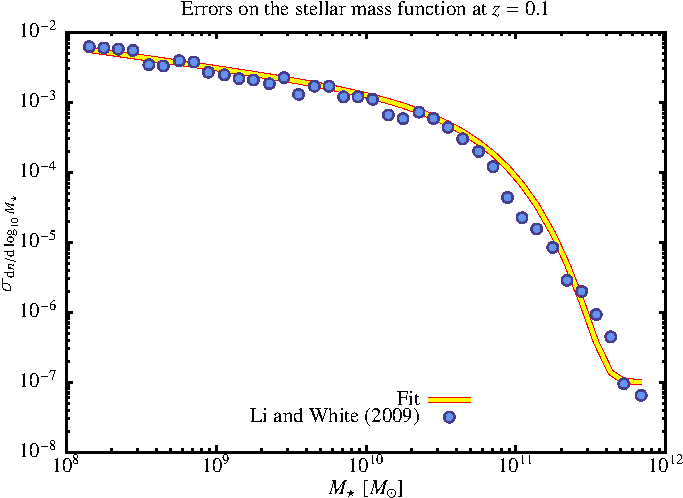
\includegraphics[width=160mm]{../plots/stellarMassFunctionErrors_z01.pdf}
 \end{center}
 \caption{Errors on the \protect\cite{li_distribution_2009} stellar mass funtion (points) and the fitting function (line) given by eqn.~(\protect\ref{eq:stellarMassFunctionErrorsFit}).}
 \label{fig:stellarMassFunctionErrors}
\end{figure}

\begin{figure}
 \begin{center}
 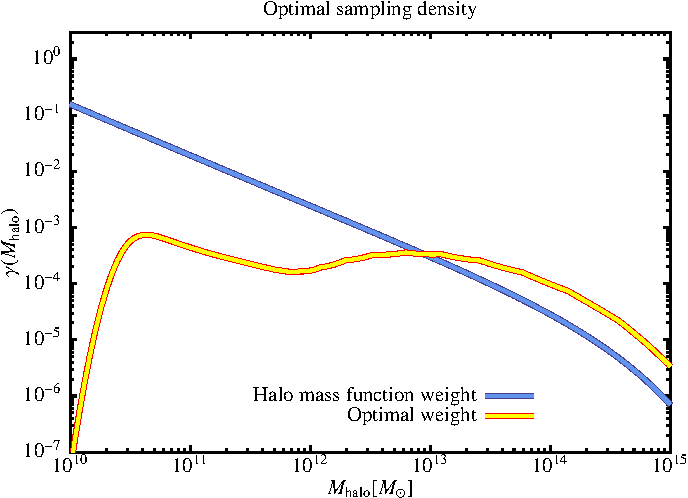
\includegraphics[width=160mm]{../plots/optimalSamplingStellarMassFunction.pdf}
 \end{center}
 \caption{Optimal weighting (yellow line) compared with weighting by the dark matter halo mass function (i.e. sampling halos at random from a representative volume; blue line). Sampling densities have been normalized to unit compute time.}
 \label{fig:optimalSamplingStellarMassFunction}
\end{figure}

\subsection{Refining by Other Merger Tree Statistics}

Since building merger trees is relatively fast, while solving the baryonic physics is slow it may be advantageous to  non-uniformly sample the distribution of merger trees at fixed merger tree mass, $M$. For example, we could assign some measure of formation history to each merger tree, such as the time since the last major merger, $\tau$. The halo mass function then becomes $n(M,\tau)$ (which can be computed by simulating large numbers of trees), and the tree sampling function becomes $\gamma(M,\tau)$. We'd then need to know the stellar mass function conditioned on both $M$ and $\tau$, $\phi_\star(M_\star|M,\tau)$. Given these, the above approach could be easily generalized to determine an optimal $\gamma(M,\tau)$. Then, after generating a merger tree, we'd first compute $\tau$. If a sufficient number of trees in that $\tau$ interval had already been computed, then we'd simply drop that tree and compute another one. The speed up here would depend on how fast building trees is relative to solving baryonic physics and what fraction of trees you discard. In principle, the trees could be generated, sampled and stored in advance so that we'd already have an optimally distributed set of trees in $M$ and $\tau$ that could be used for each model run.

\section{Constraints}\label{sec:ConstraintScripts}

Any constraint which can be applied to \glc\ is defined by two files, a configuration file and a likelihood script, which must be placed in {\normalfont \ttfamily constraints/constraints} and {\normalfont \ttfamily constraints/scripts} respectively. 

\subsection{Configuration File}\label{sec:ConstraintConfigFiles}

The configuration file should have the form:
\begin{verbatim}
<!-- Defines a constraint to match some data. -->                                          
<constraint>                                                                                                         
  <name>Long-form name of this constraint</name>                                                                      
  <label>shortLabelForThisConstraint</label>                                                                        
  <outputRedshift>0.07</outputRedshift>                                                                              
  <outputRedshift>1.00</outputRedshift>                                                                              
  <haloMassResolution>5.0e9</haloMassResolution>                                                                     
  <haloMassMinimum>2.0e10</haloMassMinimum>                                                                          
  <haloMassMaximum>2.0e14</haloMassMaximum>                                                                          
  <analysis>constraints/scripts/myAnalysisScript.pl</analysis>                                         
  <luminosity>
    <filter>UKIRT_K</filter>
    <redshift>0.0</redshift>
    <frame>rest</frame>
  </luminosity>
  <luminosity>
    <filter>UKIRT_K</filter>
    <redshift>1.0</redshift>
    <frame>observed</frame>
  </luminosity>
  <optionOn>outputMainBranchStatus</optionOn>
  <optionOn>outputDensityContrastData</optionOn>
  <parameter>
   <name>outputDensityContrastValues</name>
   <value>200.0</value>
   <accumulation>unique</accumulation>
  </parameter>
</constraint>                                                                                                        
\end{verbatim}
The {\normalfont \ttfamily name} and {\normalfont \ttfamily label} are used to describe the constraint ({\normalfont \ttfamily label} is used as a suffix in file names so should not contain spaces or other characters which might cause problems in file names). 

The remaining elements describe the requirements for this constraint. {\normalfont \ttfamily haloMassResolution} specifies the maximum resolution in mergers trees that still allows this constraint to be computed accurately. Similarly, {\normalfont \ttfamily haloMassMinimum} and {\normalfont \ttfamily haloMassMaximum} specify the required range of halo masses to simulate to allow this constraint to be computed accurately.

One or more {\normalfont \ttfamily outputRedshift} elements may be present, each specifying a redshift at which output is required for this constraint. Similarly, one or more {\normalfont \ttfamily luminosity} elements may be present, each of which specifies a luminosity which must be computed for this constraint. Each {\normalfont \ttfamily luminosity} must contain a specification of {\normalfont \ttfamily filter}, {\normalfont \ttfamily redshift}, and {\normalfont \ttfamily frame} to define which luminosity is to be computed.

One or more {\normalfont \ttfamily optionOn} elements may be present. Each element must specify the name of a \glc\ input parameter. That parameter will be set to {\normalfont \ttfamily true} in the \glc\ input parameter file.

Finally, arbitrary other parameter may be set using the standard {\normalfont \ttfamily parameter} element which should give the {\normalfont \ttfamily name} and {\normalfont \ttfamily value} for the parameter. Optionally, an {\normalfont \ttfamily accumulation} element may also be specified for each {\normalfont \ttfamily parameter}. This controls how values of the parameter are to be accumulated if set by more than one constraint. An accumulation of {\normalfont \ttfamily overwrite} will simply overwrite any previously set values. An accumulation of {\normalfont \ttfamily combine} will concatenate all values set by different constraints. Finally, an accumulation of {\normalfont \ttfamily unique} will concatenate all values set by different constraints and then filter out any duplicates.

When multiple constraints are used, their requirements are automatically combined.

\subsection{Likelihood Script}

The likelihood script for a constraint is required to perform several tasks, controlled by command line options. The script should accept the following command line syntax:
\begin{verbatim}
 myScript.pl <galacticusFile> [options...]
\end{verbatim}
where {\normalfont \ttfamily galacticusFile} is the file name of the \glc\ model for which the likelihood calculation should be performed. The following options must be supported by the script:
\begin{description}
 \item [{\normalfont \ttfamily --plotFile <fileName>}] If this option is present, the script should generate a plot showing the constraint and the model result and write it to {\normalfont \ttfamily fileName}.
 \item [{\normalfont \ttfamily --outputFile <fileName>}] If this option is present, the script should compute the log-likelihood of the model given the constraint and write it to {\normalfont \ttfamily fileName} using the format
\begin{verbatim}
 <constraint>
  <logLikelihood>-123</logLikelihood>
 </constraint>
\end{verbatim}
 \item [{\normalfont \ttfamily --accuracyFile <fileName>}] If this option is present, the script should write an XML file giving details of the accuracy of the model results relative to the observational errors using the format
\begin{verbatim}
 <accuracy>
  <x>...</x>
  .
  .
  .
  <x>...</x>
  <yModel>...</yModel>
  .
  .
  .
  <yModel>...</yModel>
  <yData>...</yData>
  .
  .
  .
  <yData>...</yData>
  <errorModel>...</errorModel>
  .
  .
  .
  <errorModel>...</errorModel>
  <errorData>...</errorData>
  .
  .
  .
  <errorData>...</errorData>
 </accuracy>
\end{verbatim}
In this file the {\normalfont \ttfamily yModel} and {\normalfont \ttfamily yData} elements should give the values of the model result and the comparable data respectively, while {\normalfont \ttfamily errorModel} and {\normalfont \ttfamily errorData} should give an estimate of the errors on these quantities. In the case of the model error this should include only the contribution arising from the finite number of merger trees simulated. This file will be used to judge whether the model is running sufficient merger trees such that the likelihood is not dominated by these errors. The {\normalfont \ttfamily x} elements are optional but can be used to give the parameter values associated with each model result.
 \item [{\normalfont \ttfamily --resultFile <fileName>}] If this option is present, the script should write an XML file giving details of the result of the model using the format
\begin{verbatim}
 <accuracy>
  <x>...</x>
  .
  .
  .
  <x>...</x>
  <y>...</y>
  .
  .
  .
  <y>...</y>
  <error>...</error>
  .
  .
  .
  <error>...</error>
 </accuracy>
\end{verbatim}
In this file the {\normalfont \ttfamily y} elements should give the values of the model result, while the {\normalfont \ttfamily error} elements should give an estimate of the errors on these results. The error should include only the contribution arising from the finite number of merger trees simulated. This file will be used to judge whether the model result is converged with respect to various numerical parameters in \glc. The {\normalfont \ttfamily x} elements are optional but can be used to give the parameter values associated with each model result.
 \item [{\normalfont \ttfamily --modelDiscrepancies <path>}] If this option is present, the script should scan {\normalfont \ttfamily path}. For each directory found in {\normalfont \ttfamily path} the script should check for the existance of a file named {\normalfont \ttfamily discrepancy<label>.hdf5} where {\normalfont \ttfamily label} is the label given for this constraint in its configuration file (see \S\ref{sec:ConstraintConfigFiles}). If present, the model discrepancy given in that file should be applied to the likelihood calculation. See \S\ref{sec:ModelDiscrepancy} for a description of the structure of the discrepancy files.
\end{description}

\subsection{Available Constraints}

\subsubsection{Methodology for Mass Functions}

In general, for constraints corresponding to mass functions (whether stellar mass or HI mass), the covariance matrix of the observational data is determined using the analytic model of \cite{smith_how_2012}. This requires knowledge of both the survey geometry (angular mask and radial extent as a function of mass) and of the \gls{hod} of the observed galaxies.

Details of the survey geometry and depth are given for each individual constraints. Computing the large-scale structure contribution to the covariance function requires integration of the non-linear matter power spectrum over the Fourier transform of the survey window function. We use the method of \cite{peacock_non-linear_1996} to determine the non-linear matter power spectrum, because of its simplicity and speed. We have checked that using a more accurate non-linear matter power spectrum (e.g. \citealt{lawrence_coyote_2010}) makes negligible difference to our results. If the angular power spectrum of the survey mask is available\footnote{Typically if the survey geometry is defined by \protect\gls{mangle} polygons, allowing the angular power spectrum to be found using the \protect\gls{mangle} {\normalfont \ttfamily harmonize} utility.}, this is used to compute the relation
\begin{equation}
  \sigma^2(M_\mu,M_\nu) = {2 \over \pi V_\mu V_\nu}\int_0^\infty {\mathrm d} k\, k^{-4} P(k) \sum_i \sum_j \sum_{\ell=0}^\infty (2\ell+1) C^{ij}_\ell R^i_{\ell}(kr_{\mu 0},kr_{\mu 1}) R^j_{\ell}(kr_{\nu 0},kr_{\nu 1}),
\end{equation}
where $(2\ell+1) C^{ij}_\ell = \sum_{m=-\ell}^{+\ell} \Psi^i_{\ell m} \Psi^{j*}_{\ell m}$, $\Psi^i_{\ell m}$ are the spherical harmonic coefficients of the $i^{\mathrm th}$ field of the survey, $V$ is the maximum distance to which a galaxy of mass $M$ can be seen, $P(k)$ is the nonlinear power spectrum and
\begin{equation}
 R_{\ell}(x_0,x_1) \equiv \int_{x_0}^{x_1} x^2 j_\ell(x) {\mathrm d}x = \sqrt{\pi} 2^{-2-\ell} \Gamma\left({1\over 2}[3+\ell]\right) \left[ x^{3+\ell} \tensor*[_1]{\stackrel{\sim}{F}}{_2} \left({1\over 2}[3+\ell]; \ell+{3\over 2},{1\over 2}(5+\ell);-{x^2\over 4}\right)\right]_{x_0}^{x_1},
\end{equation}
where $\tensor*[_1]{\stackrel{\sim}{F}}{_2}$ is the regularized generalized hypergeometric function. In other cases, where the angular power spectrum is not available, the survey geometry is realized on a grid which is when Fourier transformed to obtain the appropriate window function.

To find a suitable \gls{hod} to describe the observed galaxies we adopt the model of \cite{behroozi_comprehensive_2010}. This is an 11 parameter model which describes separately the numbers of satellite and central galaxies occupying a halo of given mass---the reader is referred to \cite{behroozi_comprehensive_2010} for a complete description of the functional form of this parametric \gls{hod}. An \gls{mcmc} approach is used to to constrain the \gls{hod} parameters to fit the observational data. We use a likelihood
\begin{equation}
 \ln \mathcal{L} = -{1\over 2} \Delta\cdot \mathcal{C}^{-1}\cdot \Delta^{\mathrm T} - {N \over 2} \ln(2\pi) - {\ln |\mathcal{C}| \over 2},
\end{equation}
where $N$ is the number of bins in the mass function, $\mathcal{C}$ is the covariance matrix of the observed mass function, and $\Delta_i = \phi_i^{\mathrm (HOD)} - \phi_i^{\mathrm (observed)}$. Of course, it is precisely this covariance matrix, $\mathcal{C}$, that we are trying to compute. We therefore adopt an iterative approach as follows:
\begin{enumerate}
 \item make an initial estimate of the covariance matrix, assuming that only Poisson errors contribute (the covariance matrix is therefore diagonal, and the terms are easily computed from the measured mass function and the survey volume as a function of stellar mass);
 \item find the maximum likelihood parameters of the \gls{hod} given the observed mass function and the current estimate of the covariance matrix;
 \item using this \gls{hod} and the framework of \cite{smith_how_2012}, compute a new estimate of the covariance matrix, including all three contributions;
 \item repeat steps 2 and 3 until convergence in the covariance matrix is achieved.
\end{enumerate}
In practice we find that this procedure often leads to an \gls{hod} and covariance matrix which oscillate between two states in successive iterations. The differences in the covariance matrix are relatively small however, so we choose to conservatively adopt the covariance matrix with the larger values.

\subsubsection{Methodology for Correlation Functions}

For constraints corresponding to (possibly, projected) correlation functions, the model expectation is computed using the halo model \cite{cooray_halo_2002}. For each model halo, each galaxy (satellite and central) is assessed to see if it meets the criteria for inclusion in the sample. Where the sample includes mass limits (either just a lower limit, or lower and upper limits) each galaxy is assigned a probability of inclusion in the sample based on its mass and the random error in mass. Thus, each halo is characterized by the probability of having a central galaxy in the sample, $p^{\mathrm (c)}$, and $N$ probabilities, $p_i^{\mathrm (s)}$, of each satellite galaxy being in the sample. We assume binomial statistics for each galaxy's probability of inclusion, and further assume that these probabilities are uncorrelated. Therefore, the contribution of the halo to the one- and two-halo terms of the power spectrum in the halo model are:
\begin{equation}
\Delta P^{\mathrm 1h}(k) = {w \over n_{\mathrm gal}^2} \left[ p^{\mathrm (c)} \sum_{i=1}^N p^{\mathrm (s)} u(k|M) + \sum_{k=0}^N k(k-1) P\left(p_i^{\mathrm (s)},\ldots,p_N^{(s)}\right) u(k|M)^2 \right]
\end{equation}
and
\begin{equation}
\Delta \sqrt{P^{\mathrm 2h}}(k) = {w \over n_{\mathrm gal}} \sqrt{P^{\mathrm lin}}(k) b(M) u(k|M) \left[ p^{\mathrm (c)} + \sum_{i=1}^N p_i^{\mathrm (s)} \right],
\end{equation}
respectively, where $w$ is the weight of the halo (i.e. the number of such model halos expected per unit volume), $b(M)$ is the bias of halos of mass $M$, $u(k|M)$ is the Fourier-transform of the halo density profile, and $P_{\mathrm lin}(k)$ is the linear theory power spectrum, and $P(p_1,\ldots,p_N)$ is the Poisson binomial distribution for $N$ events with probabities $p_1,\ldots,p_N$. The contribution of the halo to the galaxy density, $n_{\mathrm gal}$, is simply $\Delta n_{\mathrm gal} = w \left[ p^{\mathrm (c)} + \sum_{i=1}^N p_i^{\mathrm (s)} \right]$.

\subsubsection{Li \& White (2009) SDSS Stellar Mass Function}

This constraint utilizes the stellar mass function for $z\approx 0.07$ galaxies measured by \cite{li_distribution_2009} from the \gls{sdss}. The mass function reported by \cite{li_distribution_2009} is converted to the appropriate Hubble constant for the given \glc\ model (assuming that masses scale as $H_0^{-2}$ and volumes as $H_0^3$)---no adjustment is made for cosmological parameters given the low redshift of the sample.

Given a \glc\ model, total stellar masses of model galaxies are adjusted using:
\begin{equation}
 M_\star \rightarrow {\mathbf G} {\mathbf S} M_\star 
\end{equation}
where the ${\mathbf S}$ operator is a multiplicative factor accounting for systematic errors in stellar mass determination and is equal to \citep{behroozi_comprehensive_2010}
\begin{equation}
 \log_{\mathrm 10} S = \mu + \kappa \log_{\mathrm 10} \left({M_\star \over 10^{11.3}M_\odot}\right)
\end{equation}
where $\mu=${\normalfont \ttfamily [sdssStellarMassFunctionZ0.07StellarMassSystematicMu]}, $\kappa=${\normalfont \ttfamily [sdssStellarMassFunctionZ0.07StellarMassSystematiKappa]}, and the {\normalfont \bfseries G} operator is a multiplicative factor drawn from a log-normal distribution of width $0.07$~dex for each galaxy to mimic the effects of random errors on stellar masses (motivated by the discussion of \cite{behroozi_comprehensive_2010}).

The model masses are then used to construct a mass function by binning into a histogram using the masses reported by \cite{li_distribution_2009} (modified as described above) as the centers of the bins (with bin boundaries placed at the geometric means of consecutive bin centers).

If the {\normalfont \ttfamily --modelDiscrepancies} option is given, then any multiplicative or additive discrepancies found are applied to the model mass function, and any additional covariance is added to the covariance matrix.

The covariance matrix is computed as
\begin{equation}
 {\mathbf C} = {\mathbf C}_{\mathrm obs} + {\mathbf C}_{\mathrm model,random} + \sum_i {\mathbf C}_{{\mathrm discrepancy}, i},
\end{equation}
where ${\mathbf C}_{\mathrm obs}$ is the covariance matrix of the observational data, ${\mathbf C}_{\mathrm model,random}$ is the covariance matrix of the model arising from random noise (due to the finite number of trees simulated---see \S\ref{sec:AnalysisALFALFAHIMassFunction} for a description of how this covariance matrix is estimated), and ${\mathbf C}_{{\mathrm discrepancy}, i}$ is the covariance due to the $i^{\mathrm th}$ model discrepancy.

The model likelihood is then computed using:
\begin{equation}
 \mathcal{L} = {1 \over \sqrt{(2 \pi)^n |{\mathbf C}|}} \exp\left[ -{1\over 2} \Delta {\mathbf C}^{-1} \Delta \right],
\end{equation}
where $\Delta_i = \Phi_{{\mathrm model}, i} - \Phi_{{\mathrm observed}, i}$ is the difference between the model and observed mass functions, and $n$ is the number of points in the mass function histogram.

\subsubsection{Caputi et al. (2011) UKIDSS UDS Stellar Mass Function}\label{sec:ConstraintsUKIDSSUDSStellarMassFunction}

This constraint utilizes the stellar mass functions for $z = 3$ to 5 galaxies measured by \cite{caputi_stellar_2011} from the UKISS UDS survey.  If the {\normalfont \ttfamily --modelDiscrepancies} option is given, then any multiplicative or additive discrepancies found are applied to the model mass function, and any additional covariance is added to the covariance matrix.

Given a \glc\ model, total stellar masses of model galaxies are adjusted using:
\begin{equation}
 M_\star \rightarrow {\mathbf G} {\mathbf S} M_\star 
\end{equation}
where the ${\mathbf S}$ operator is a multiplicative factor accounting for systematic errors in stellar mass determination and is equal to \citep{behroozi_comprehensive_2010}
\begin{equation}
 \log_{\mathrm 10} S = \mu + \kappa \log_{\mathrm 10} \left({M_\star \over 10^{11.3}M_\odot}\right)
\end{equation}
where $\mu=${\normalfont \ttfamily [ukidssUdsStellarMassFunctionZX.XXXStellarMassSystematicMu]}, $\kappa=${\normalfont \ttfamily [ukidssUdsStellarMassFunctionZX.XXXStellarMassSystematiKappa]}, and the {\normalfont \bfseries G} operator is a multiplicative factor drawn from a log-normal distribution of width $0.173$~dex for each galaxy to mimic the effects of random errors on stellar masses (which accounts for errors in photometric redshifts, $\delta z/(1+z)$ of $\sigma=0.05$ as reported by \cite{caputi_stellar_2011} along with an additional 0.087~dex added in quadrature to account for SED fitting errors, judged from Figure 8 of \cite{caputi_stellar_2011}).

The covariance matrix is computed as
\begin{equation}
 {\mathbf C} = {\mathbf C}_{\mathrm obs} + {\mathbf C}_{\mathrm model,random} + \sum_i {\mathbf C}_{{\mathrm discrepancy}, i},
\end{equation}
where ${\mathbf C}_{\mathrm obs}$ is the covariance matrix of the observational data, ${\mathbf C}_{\mathrm model,random}$ is the covariance matrix of the model arising from random noise (due to the finite number of trees simulated, and ${\mathbf C}_{{\mathrm discrepancy}, i}$ is the covariance due to the $i^{\mathrm th}$ model discrepancy.

The model likelihood is then computed using:
\begin{equation}
 \mathcal{L} = {1 \over \sqrt{(2 \pi)^n |{\mathbf C}|}} \exp\left[ -{1\over 2} \Delta {\mathbf C}^{-1} \Delta \right],
\end{equation}
where $\Delta_i = \Phi_{{\mathrm model}, i} - \Phi_{{\mathrm observed}, i}$ is the difference between the model and observed mass functions, and $n$ is the number of points in the mass function histogram.

The survey window function is determined from the set of galaxy positions provided by Caputi (private communication), by finding a suitable bounding box and then cutting out empty regions (corresponding to regions that were removed around bright stars). A set of random points are then found within this mask and are used to find the Fourier transform of the survey volume. 

To estimate the depth of the \cite{caputi_stellar_2011} sample as a function of galaxy stellar mass we make use of semi-analytic models in the Millennium Database. Specifically, we use the \glspl{sam} of \cite{guo_dwarf_2011} and \cite{henriques_confronting_2012} specifically the {\normalfont \ttfamily Guo2010a..MR} and {\normalfont \ttfamily Henriques2012a.wmap1.BC03\_001} tables in the Millennium Database. For each snapshot in the database, we extract the stellar masses and observed-frame IRAC 4.5$\mu$m apparent magnitudes (including dust extinction), and determine the median apparent magnitude as a function of stellar mass. Using the limiting apparent magnitude of the \cite{caputi_stellar_2011} sample, $i_{4.5}=24$, we infer the corresponding absolute magnitude at each redshift and, using our derived apparent magnitude--stellar mass relation, infer the corresponding stellar mass.

The end result of this procedure is the limiting stellar mass as a function of redshift, accounting for k-corrections, evolution, and the effects of dust. Figure~\ref{fig:UKIDSSUDSMassRedshift} shows the resulting relation between stellar mass and the maximum redshift at which such a galaxy would be included in the sample. Points indicate measurements from the \gls{sam}, while the line shows a polynomial fit:
\begin{equation}
 z(M_\star) = -56.247 + 5.881 m,
 \label{eq:UKIDSSUDSDepthPolynomial}
\end{equation}
where $m= \log_{10}(M_\star/M_\odot)$. We use this polynomial fit to determine the depth of the sample as a function of stellar mass.

\begin{figure}
 \begin{center}
 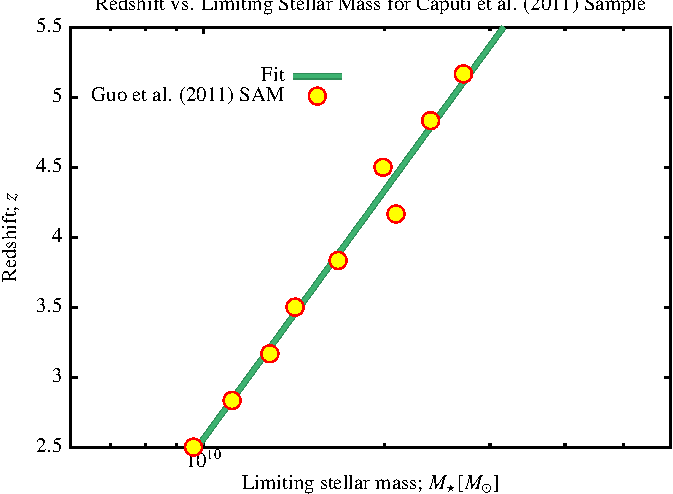
\includegraphics[width=85mm,trim=0mm 0mm 0mm 4mm,clip]{Plots/DataAnalysis/UKIDSSUDSMassLuminosityRelation.pdf}
 \caption{The maximum redshift at which a galaxy of given stellar mass can be detected in the sample of \protect\cite{caputi_stellar_2011}. Points show the results obtained using the \protect\cite{henriques_confronting_2012} model from the Millennium Database, while the lines shows a polynomial fit to these results (given in eqn.~\ref{eq:UKIDSSUDSDepthPolynomial}).}
 \end{center}
 \label{fig:UKIDSSUDSMassRedshift}
\end{figure}

Finally, the incompleteness of the observational sample (which is required when estimating the Poisson contribution to the covariance matrix) is found from the 50\% and 80\% completeness masses, $M_{50}$ and $M_{80}$ respectively, given in Fig.~4 of \cite{caputi_stellar_2011}. Specifically, we assume that, at a given mass $M$, the number of photons being received from a galaxy can be modeled as a Gaussian distribution with mean $f M$ and variance $fM+\mu$, where $\mu$ is the number of photons ariving from the sky. The fraction of sources of mass $M$ that will be detected at more than $n \sigma$ above the background is then
\begin{eqnarray}
f(M) & = & \int_{n\sqrt{mu}}^\infty {1 \over \sqrt{2 \pi} \sqrt{f M + \mu}} \exp\left( - {[S-fM]^2 \over 2 [f M + \mu]} \right) {\mathrm d}S \nonumber \\
     & = & {1 \over 2}\left[ 1 - \hbox{erf}\left( {x(M) \over \sqrt{2}} \right)  \right],
\label{eq:incompleteness}
\end{eqnarray}
where $x(M) = (n \sqrt{mu} - f M)/(\mu+fM)^{1/2}$. Given $f(M_{\mathrm 50})=0.5$ and $f(M_{\mathrm 80})=0.8$ we can solve for $f$ and $\mu$, and then compute the completeness in each mass using eqn.~(\ref{eq:incompleteness}). The resulting completeness curves are shown in Fig.~\ref{fig:UKIDSSUDSCompleteness}. Note that the model of eqn.~(\ref{eq:incompleteness}) is clearly an oversimplification, but should capture the expected behavior of the completeness and, since it is fit to the 50\% and 80\% completenesses reported by \cite{caputi_stellar_2011}---which were computed using detailed simulations---should work sufficiently well.

\begin{figure}
 \begin{center}
 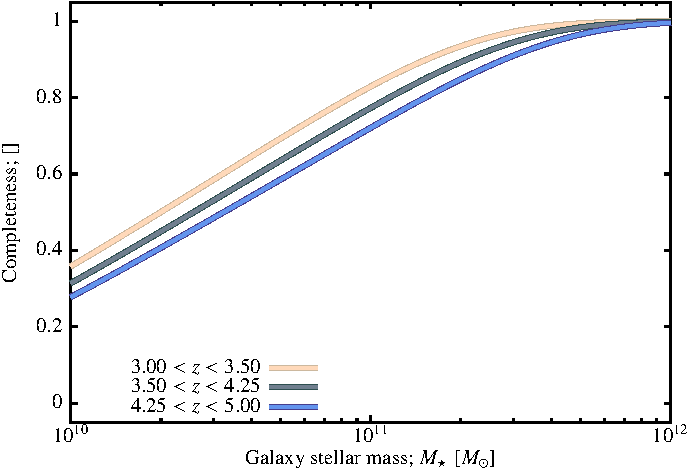
\includegraphics[width=85mm,trim=0mm 0mm 0mm 4mm,clip]{Plots/DataAnalysis/UKIDSSUDSCompleteness.pdf}
 \caption{The completeness as a function of stellar mass in the survey of \protect\cite{caputi_stellar_2011}. Curves are computed using eqn.~(\protect\ref{eq:incompleteness}) with parameters fit to the reported 50\% and 80\% completeness masses from \protect\cite{caputi_stellar_2011}.}
 \end{center}
 \label{fig:UKIDSSUDSCompleteness}
\end{figure}

\subsubsection{Bernardi et al. (2013) SDSS Stellar Mass Function}\label{sec:AnalysisBernardiSDSSStellarMassFunction}

This constraint utilizes the stellar mass function for $z\approx 0.07$ galaxies measured by \cite{bernardi_massive_2013} from the SDSS survey. The mass function, and its covariance matrix ${\mathbf C}_{\mathrm model}$, is calculated as described in \S\ref{sec:otfAnalysis:ALFALFA}, typically on-the-fly as \glc\ is run. If the {\normalfont \ttfamily --modelDiscrepancies} option is given, then any multiplicative or additive discrepancies found are applied to the model mass function, and any additional covariance is added to the covariance matrix.

The covariance matrix is computed as
\begin{equation}
 {\mathbf C} = {\mathbf C}_{\mathrm obs} + {\mathbf C}_{\mathrm model,random} + \sum_i {\mathbf C}_{{\mathrm discrepancy}, i},
\end{equation}
where ${\mathbf C}_{\mathrm obs}$ is the covariance matrix of the observational data, ${\mathbf C}_{\mathrm model,random}$ is the covariance matrix of the model arising from random noise (due to the finite number of trees simulated, and ${\mathbf C}_{{\mathrm discrepancy}, i}$ is the covariance due to the $i^{\mathrm th}$ model discrepancy.

The model likelihood is then computed using:
\begin{equation}
 \mathcal{L} = {1 \over \sqrt{(2 \pi)^n |{\mathbf C}|}} \exp\left[ -{1\over 2} \Delta {\mathbf C}^{-1} \Delta \right],
\end{equation}
where $\Delta_i = \Phi_{{\mathrm model}, i} - \Phi_{{\mathrm observed}, i}$ is the difference between the model and observed mass functions, and $n$ is the number of points in the mass function histogram.

When computing the Poisson term in the covariance matrix, the number of galaxies per bin is determined directly from the mass function, assuming a 91\% completeness\footnote{7\% arising from fiber collisions, 2\% from failures in the Pymorph pipeline (M.~Bernardi, private communication).}. The survey geometry and depth is described in \S\ref{phys:surveyGeometry:surveyGeometryBernardi2013SDSS}.

\subsubsection{Baldry et al. (2012) GAMA Stellar Mass Function}\label{sec:AnalysisBaldryGAMAStellarMassFunction}

This constraint utilizes the stellar mass function for $z< 0.06$ galaxies measured by \cite{baldry_galaxy_2012} from the GAMA survey. The mass function, and its covariance matrix ${\mathbf C}_{\mathrm model}$, is calculated as described in \S\ref{sec:otfAnalysis:ALFALFA}, typically on-the-fly as \glc\ is run. If the {\normalfont \ttfamily --modelDiscrepancies} option is given, then any multiplicative or additive discrepancies found are applied to the model mass function, and any additional covariance is added to the covariance matrix.

The covariance matrix is computed as
\begin{equation}
 {\mathbf C} = {\mathbf C}_{\mathrm obs} + {\mathbf C}_{\mathrm model,random} + \sum_i {\mathbf C}_{{\mathrm discrepancy}, i},
\end{equation}
where ${\mathbf C}_{\mathrm obs}$ is the covariance matrix of the observational data, ${\mathbf C}_{\mathrm model,random}$ is the covariance matrix of the model arising from random noise (due to the finite number of trees simulated, and ${\mathbf C}_{{\mathrm discrepancy}, i}$ is the covariance due to the $i^{\mathrm th}$ model discrepancy.

The model likelihood is then computed using:
\begin{equation}
 \mathcal{L} = {1 \over \sqrt{(2 \pi)^n |{\mathbf C}|}} \exp\left[ -{1\over 2} \Delta {\mathbf C}^{-1} \Delta \right],
\end{equation}
where $\Delta_i = \Phi_{{\mathrm model}, i} - \Phi_{{\mathrm observed}, i}$ is the difference between the model and observed mass functions, and $n$ is the number of points in the mass function histogram.

When computing the Poisson term in the covariance matrix, the number of galaxies per bin is taken from data supplied by I.~Baldry (private communication). The survey geometry and depth is described in \S\ref{phys:surveyGeometry:surveyGeometryBaldry2012GAMA}.

Finally, the completeness of the observational sample is estimated to be greater than 98\% (P.~Norberg, private communication). Therefore we add an additional contribution to the observed covariance matrix equal to $\mathcal{C}_{ij} = 0.02 \phi_i \phi_j$ where $\phi$ is the observed mass function.

\subsubsection{Tomczak et al. (2014) ZFOURGE Stellar Mass Functions}\label{sec:AnalysisTomczakZFOURGEStellarMassFunction}

This constraint utilizes the stellar mass function for $0.2 < z< 3$ galaxies measured by \cite{tomczak_galaxy_2014} from the ZFOURGE survey. The mass function, and its covariance matrix ${\mathbf C}_{\mathrm model}$, is calculated as described in \S\ref{sec:otfAnalysis:ALFALFA}, typically on-the-fly as \glc\ is run. If the {\normalfont \ttfamily --modelDiscrepancies} option is given, then any multiplicative or additive discrepancies found are applied to the model mass function, and any additional covariance is added to the covariance matrix.

The covariance matrix is computed as
\begin{equation}
 {\mathbf C} = {\mathbf C}_{\mathrm obs} + {\mathbf C}_{\mathrm model,random} + \sum_i {\mathbf C}_{{\mathrm discrepancy}, i},
\end{equation}
where ${\mathbf C}_{\mathrm obs}$ is the covariance matrix of the observational data, ${\mathbf C}_{\mathrm model,random}$ is the covariance matrix of the model arising from random noise (due to the finite number of trees simulated, and ${\mathbf C}_{{\mathrm discrepancy}, i}$ is the covariance due to the $i^{\mathrm th}$ model discrepancy.

The model likelihood is then computed using:
\begin{equation}
 \mathcal{L} = {1 \over \sqrt{(2 \pi)^n |{\mathbf C}|}} \exp\left[ -{1\over 2} \Delta {\mathbf C}^{-1} \Delta \right],
\end{equation}
where $\Delta_i = \Phi_{{\mathrm model}, i} - \Phi_{{\mathrm observed}, i}$ is the difference between the model and observed mass functions, and $n$ is the number of points in the mass function histogram.

When computing the Poisson term in the covariance matrix, the number of galaxies per bin is taken directly from tables provided by R.~Quadri (private communication).

\subsubsection{Davidzon et al. (2013) VIPERS Stellar Mass Functions}\label{sec:AnalysisDavidzonVIPERSStellarMassFunction}

This constraint utilizes the stellar mass function for $0.5 < z< 1.0$ galaxies measured by \cite{davidzon_vimos_2013} from the VIPERS survey. The mass function, and its covariance matrix ${\mathbf C}_{\mathrm model}$, is calculated as described in \S\ref{sec:otfAnalysis:ALFALFA}, typically on-the-fly as \glc\ is run. If the {\normalfont \ttfamily --modelDiscrepancies} option is given, then any multiplicative or additive discrepancies found are applied to the model mass function, and any additional covariance is added to the covariance matrix.

The covariance matrix is computed as
\begin{equation}
 {\mathbf C} = {\mathbf C}_{\mathrm obs} + {\mathbf C}_{\mathrm model,random} + \sum_i {\mathbf C}_{{\mathrm discrepancy}, i},
\end{equation}
where ${\mathbf C}_{\mathrm obs}$ is the covariance matrix of the observational data, ${\mathbf C}_{\mathrm model,random}$ is the covariance matrix of the model arising from random noise (due to the finite number of trees simulated, and ${\mathbf C}_{{\mathrm discrepancy}, i}$ is the covariance due to the $i^{\mathrm th}$ model discrepancy.

The model likelihood is then computed using:
\begin{equation}
 \mathcal{L} = {1 \over \sqrt{(2 \pi)^n |{\mathbf C}|}} \exp\left[ -{1\over 2} \Delta {\mathbf C}^{-1} \Delta \right],
\end{equation}
where $\Delta_i = \Phi_{{\mathrm model}, i} - \Phi_{{\mathrm observed}, i}$ is the difference between the model and observed mass functions, and $n$ is the number of points in the mass function histogram.

When computing the Poisson term in the covariance matrix, the number of galaxies per bin is taken directly from tables supplied by I.~Davidzon (private communication).

\subsubsection{Muzzin et al. (2013) ULTRAVISTA Stellar Mass Functions}\label{sec:AnalysisMuzzinULTRAVISTAStellarMassFunction}

This constraint utilizes the stellar mass function for $0.2 < z< 4.0$ galaxies measured by \cite{muzzin_evolution_2013} from the ULTRAVISTA survey. The mass function, and its covariance matrix ${\mathbf C}_{\mathrm model}$, is calculated as described in \S\ref{sec:otfAnalysis:ALFALFA}, typically on-the-fly as \glc\ is run. If the {\normalfont \ttfamily --modelDiscrepancies} option is given, then any multiplicative or additive discrepancies found are applied to the model mass function, and any additional covariance is added to the covariance matrix.

The covariance matrix is computed as
\begin{equation}
 {\mathbf C} = {\mathbf C}_{\mathrm obs} + {\mathbf C}_{\mathrm model,random} + \sum_i {\mathbf C}_{{\mathrm discrepancy}, i},
\end{equation}
where ${\mathbf C}_{\mathrm obs}$ is the covariance matrix of the observational data, ${\mathbf C}_{\mathrm model,random}$ is the covariance matrix of the model arising from random noise (due to the finite number of trees simulated, and ${\mathbf C}_{{\mathrm discrepancy}, i}$ is the covariance due to the $i^{\mathrm th}$ model discrepancy.

The model likelihood is then computed using:
\begin{equation}
 \mathcal{L} = {1 \over \sqrt{(2 \pi)^n |{\mathbf C}|}} \exp\left[ -{1\over 2} \Delta {\mathbf C}^{-1} \Delta \right],
\end{equation}
where $\Delta_i = \Phi_{{\mathrm model}, i} - \Phi_{{\mathrm observed}, i}$ is the difference between the model and observed mass functions, and $n$ is the number of points in the mass function histogram.

When computing the Poisson term in the covariance matrix, the completeness is taken to be 95\% in the lowest mass bins, and 100\% in all other bins \citep{muzzin_evolution_2013}.

\subsubsection{Moustakas et al. (2013) PRIMUS Stellar Mass Functions}\label{sec:AnalysisMoustakasPRIMUSSStellarMassFunctions}

This constraint utilizes the stellar mass functions for $z\approx 0.2$ to $z\approx 1$ galaxies measured by \cite{moustakas_primus:_2013} from the PRIMUS survey. The mass functions, and their covariance matrices ${\mathbf C}_{\mathrm model}$, are calculated as described in \S\ref{sec:otfAnalysis:ALFALFA}, typically on-the-fly as \glc\ is run. If the {\normalfont \ttfamily --modelDiscrepancies} option is given, then any multiplicative or additive discrepancies found are applied to the model mass function, and any additional covariance is added to the covariance matrix.

The covariance matrix is computed as
\begin{equation}
 {\mathbf C} = {\mathbf C}_{\mathrm obs} + {\mathbf C}_{\mathrm model,random} + \sum_i {\mathbf C}_{{\mathrm discrepancy}, i},
\end{equation}
where ${\mathbf C}_{\mathrm obs}$ is the covariance matrix of the observational data, ${\mathbf C}_{\mathrm model,random}$ is the covariance matrix of the model arising from random noise (due to the finite number of trees simulated, and ${\mathbf C}_{{\mathrm discrepancy}, i}$ is the covariance due to the $i^{\mathrm th}$ model discrepancy.

The model likelihood is then computed using:
\begin{equation}
 \mathcal{L} = {1 \over \sqrt{(2 \pi)^n |{\mathbf C}|}} \exp\left[ -{1\over 2} \Delta {\mathbf C}^{-1} \Delta \right],
\end{equation}
where $\Delta_i = \Phi_{{\mathrm model}, i} - \Phi_{{\mathrm observed}, i}$ is the difference between the model and observed mass functions, and $n$ is the number of points in the mass function histogram.

When computing the Poisson term in the covariance matrix, the number of galaxies per bin is taken directly from \cite{moustakas_primus:_2013}. The survey geometry and depth is described in \S\ref{phys:surveyGeometry:surveyGeometryMoustakas2013PRIMUS}.

\subsubsection{Martin et al. (2010) ALFALFA HI Mass Function}\label{sec:AnalysisALFALFAHIMassFunction}

This constraint utilizes the HI mass function for $z\approx 0.0$ galaxies measured by \cite{martin_arecibo_2010} from the ALFALFA survey. The mass function, and its covariance matrix ${\mathbf C}_{\mathrm model}$, is calculated as described in \S\ref{sec:otfAnalysis:ALFALFA}, typically on-the-fly as \glc\ is run. If the {\normalfont \ttfamily --modelDiscrepancies} option is given, then any multiplicative or additive discrepancies found are applied to the model mass function, and any additional covariance is added to the covariance matrix.

The covariance matrix is computed as
\begin{equation}
 {\mathbf C} = {\mathbf C}_{\mathrm obs} + {\mathbf C}_{\mathrm model,random} + \sum_i {\mathbf C}_{{\mathrm discrepancy}, i},
\end{equation}
where ${\mathbf C}_{\mathrm obs}$ is the covariance matrix of the observational data, ${\mathbf C}_{\mathrm model,random}$ is the covariance matrix of the model arising from random noise (due to the finite number of trees simulated, and ${\mathbf C}_{{\mathrm discrepancy}, i}$ is the covariance due to the $i^{\mathrm th}$ model discrepancy.

The model likelihood is then computed using:
\begin{equation}
 \mathcal{L} = {1 \over \sqrt{(2 \pi)^n |{\mathbf C}|}} \exp\left[ -{1\over 2} \Delta {\mathbf C}^{-1} \Delta \right],
\end{equation}
where $\Delta_i = \Phi_{{\mathrm model}, i} - \Phi_{{\mathrm observed}, i}$ is the difference between the model and observed mass functions, and $n$ is the number of points in the mass function histogram.

When computing the Poisson term in the covariance matrix, the number of galaxies per bin is taken directly from Fig.~5 of \cite{martin_arecibo_2010} such that incompleteness is automatically accounted for. The survey geometry and depth is described in \S\ref{phys:surveyGeometry:surveyGeometryMartin2010ALFALFA}.

The resulting maximum likelihood mass function is shown in Fig.~\ref{fig:MaximumLikelihoodMassFunctionHOD}, clearly illustrating that this parametric \gls{hod} can produce an excellent match to the observed mass function. The resulting correlation matrix is shown in Fig.~\ref{fig:CorrelationMatrixALFALFA}. As expected, at the higher masses the correlation matrix is dominated by the on-diagonal terms---arising from the Poisson fluctuations in the number of galaxies due to the scarcity of these massive systems. At lower masses the matrix has significant off-diagonal amplitude, indicating strong correlations between nearby bins, arising from both large-scale structure and halo contributions to the covariance. This structure significantly weakens the constraint arising from the low-mass end of the mass function.

\begin{figure}
 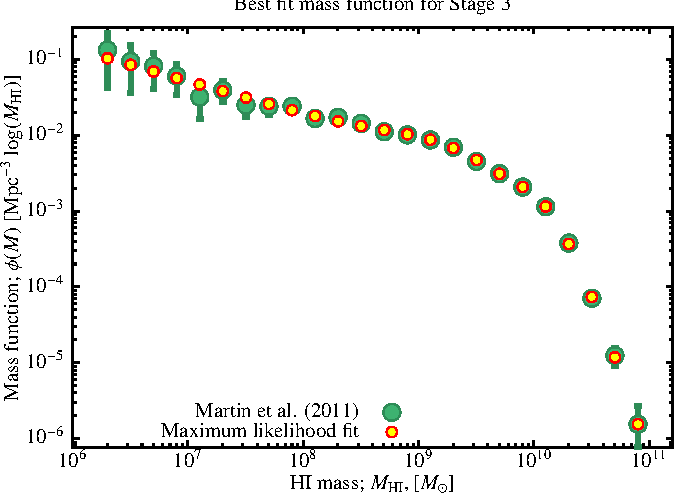
\includegraphics[width=85mm,trim=0mm 0mm 0mm 2.5mm,clip]{Plots/DataAnalysis/alfalfaHIMassFunctionBestFit.pdf}
 \caption{The maximum likelihood mass function obtained from our parametric \protect\gls{hod} (yellow points), compared to the observed HI mass function of \protect\citeauthor{martin_arecibo_2010}~(\citeyear{martin_arecibo_2010}; green points).}
 \label{fig:MaximumLikelihoodMassFunctionHOD}
\end{figure}

\begin{figure}
 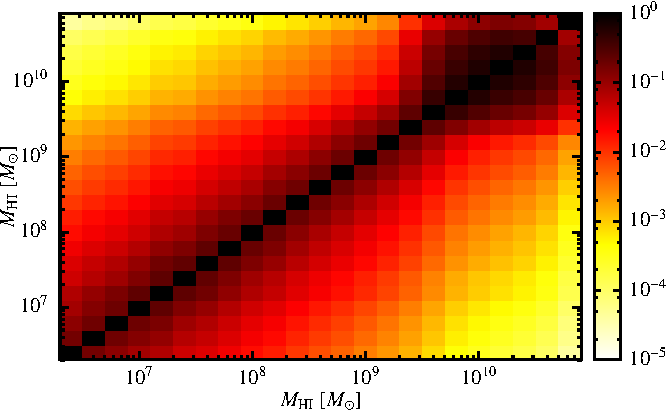
\includegraphics[width=85mm,trim=0mm 0mm 0mm 0mm,clip]{Plots/DataAnalysis/alfalfaHICorrelationmatrix.pdf}
 \caption{The correlation matrix of the observed galaxy HI mass function of \protect\cite{martin_arecibo_2010}. Color indicates the strength of correlation between bins, according to the scale shown on the right.}
 \label{fig:CorrelationMatrixALFALFA}
\end{figure}

\subsubsection{Shen et al. (2003) Late-Type Galaxy Size Distribution}\label{sec:SDSSLateTypeGalaxySizeDistribution}

This constraint utilizes the distribution of Petrosian half-light radii for $z\approx 0.07$ late-type galaxies measured by \cite{shen_size_2003} from the \gls{sdss}. The size function reported by \cite{shen_size_2003} is converted to the appropriate cosmology for the given \glc\ model (assuming that sizes scale as the angular diameter distance, and masses as the square of the luminosity distance).

Given a \glc\ model, total stellar masses of model galaxies are adjusted using:
\begin{equation}
 M_\star \rightarrow {\mathbf G} {\mathbf S} M_\star 
\end{equation}
where the ${\mathbf S}$ operator is a multiplicative factor accounting for systematic errors in stellar mass determination and is equal to \citep{behroozi_comprehensive_2010}
\begin{equation}
 \log_{\mathrm 10} S = \mu + \kappa \log_{\mathrm 10} \left({M_\star \over 10^{11.0}M_\odot}\right)
\end{equation}
where $\mu=${\normalfont \ttfamily [diskGalaxySizesSDSSZ0.07MassSystematic0]}, $\kappa=${\normalfont \ttfamily [diskGalaxySizesSDSSZ0.07MassSystematic1]}, and the {\normalfont \bfseries G} operator is a multiplicative factor drawn from a log-normal distribution of width $0.0806$~dex for each galaxy to mimic the effects of random errors on stellar masses (motivated by the statement from \cite{shen_size_2003} who quote the 95\% confidence
interval on masses as being $\pm 40$\%).

{\normalfont \bfseries Note:} This analysis currently assumes that model galaxies have disk Petrosian half-mass radii of
\begin{equation}
 R_{\mathrm 50} = 1.6676 {1 \over \sqrt{2}} \lambda R_{\mathrm vir}.
\end{equation}

Disk sizes of model galaxies are then adjusted using:
\begin{equation}
 R_{50} \rightarrow {\mathbf G} {\mathbf S} R_{50} 
\end{equation}
where the ${\mathbf S}$ operator is a multiplicative factor accounting for systematic errors in radius determination and in determination of radius from halo virial radius and spin and is equal to
\begin{equation}
 \log_{\mathrm 10} S = \mu + \kappa \log_{\mathrm 10} \left({R_{50} \over 1 \hbox{kpc}}\right)
\end{equation}
where $\mu=${\normalfont \ttfamily [iskGalaxySizesSDSSZ0.07RadiusSystematic0]}, $\kappa=${\normalfont \ttfamily [iskGalaxySizesSDSSZ0.07RadiusSystematic1]}, and the {\normalfont \bfseries G} operator is a multiplicative factor drawn from a log-normal distribution of width $0.0128$~dex for each galaxy to mimic the effects of random errors on disk radii (estimated from the fractional errors reported in the \gls{sdss} database).

The model sizes and masses are then used to construct a mass-dependent radius function by binning into a 2-D histogram using the size and mass bins reported by \cite{shen_size_2003} (modified as described above) as the centers of the bins (with bin boundaries placed at the geometric means of consecutive bin centers).

If the {\normalfont \ttfamily --modelDiscrepancies} option is given, then any multiplicative or additive discrepancies found are applied to the model mass function, and any additional covariance is added to the covariance matrix.

The covariance matrix is computed as
\begin{equation}
 {\mathbf C} = {\mathbf C}_{\mathrm obs} + {\mathbf C}_{\mathrm model,random} + \sum_i {\mathbf C}_{{\mathrm discrepancy}, i},
\end{equation}
where ${\mathbf C}_{\mathrm obs}$ is the covariance matrix of the observational data, ${\mathbf C}_{\mathrm model,random}$ is the covariance matrix of the model arising from random noise (due to the finite number of trees simulated, and ${\mathbf C}_{{\mathrm discrepancy}, i}$ is the covariance due to the $i^{\mathrm th}$ model discrepancy.

The model covariance matrix is estimated using the sample methods as described in \S\ref{sec:AnalysisALFALFAHIMassFunction}. The only difference is that in this case we have a 2-D histogram. This 2-D histogram is ``flattened'' into a 1-D vector for purposes of likelihood computation however, so covariance matrix estimation proceeds unchanged. (Note that correlations between mass bins are accounted for, in additional to correlations between radius bins.) Since the radius functions of \cite{shen_size_2003} are normalized to unity at each mass, we must account for this in the covariance matrix. The radius function transforms as:
\begin{equation}
 f_{ik} \rightarrow {f_{ik} \over \Delta \log_{10} R \sum_i f_{ik} },
\end{equation}
where $i$ indexes radius bins, $k$ indexes mass bins, and $\Delta \log_{10} R$ is the width of the radius bin. The Jacobian of this transformation is simply
\begin{equation}
 J_{ij} = {\delta_{ij} - f_i \over  \Delta \log_{10} R \sum_i f_{ik}}.
\end{equation}
Therefore, the covariance matrix is modified according to $\mathcal{C} \rightarrow J \mathcal{C} J^{\mathrm T}$. The same transformation is applied to the covariance matrix of the observed data (for which the reported errors are simply the Poisson errors on each bin).

The model likelihood is then computed using:
\begin{equation}
 \mathcal{L} = {1 \over \sqrt{(2 \pi)^n |{\mathbf C}|}} \exp\left[ -{1\over 2} \Delta {\mathbf C}^{-1} \Delta \right],
\end{equation}
where $\Delta_i = \Phi_{{\mathrm model}, i} - \Phi_{{\mathrm observed}, i}$ is the difference between the model and observed mass functions, and $n$ is the number of points in the mass function histogram.

\section{Constraint Compilations}

To specify which constraints will be applied to a particular model, a compilation file is used. These must be stored in {\normalfont \ttfamily constraints/compilations}. An example of such a file follows:
\begin{verbatim}
<constraintCompilation>
  <constraint>
    <definition>constraints/constraints/stellarMassFunction_SDSS_z0.07.xml</definition>
    <weight>1.0</weight>
  </constraint>
  <constraint>
    <definition>constraints/constraints/hiMassFunction_ALFALFA_z0.00.xml</definition>
    <weight>1.0</weight>
  </constraint>
</constraintCompilation>
\end{verbatim}
Each {\normalfont \ttfamily constraint} element specifies one constraint that will be included in this compilation, and must contain a {\normalfont \ttfamily definition} element, giving the path of the configuration file for this constraint, and a {\normalfont \ttfamily weight} element which allows the relative weight given to each constraint to be varied\footnote{Note that, if your constraints are computing correct likelihoods, re-weighting them may not be a good idea. \emph{Caveat constrainor.}}.

\section{Constraint File}

\glc\ has a complete constraints infrastructure which implements various \gls{mcmc} algorithms to analyze the posterior probability distribution of the model given some compilation of constraints. The infrastructure is \gls{mpi} parallelized and ideal for running on large compute clusters.

To perform a constraint calculation simply build the constraint code:
\begin{verbatim}
 make Constrain_Galacticus.exe
\end{verbatim}
and run with a parameter file and configuration file. Typically, you will want to run this code under \gls{mpi}, for example:
\begin{verbatim}
 mpirun -n 4 Constrain_Galacticus.exe mcmcParameters.xml mcmcConfig.xml
\end{verbatim}
would run 4 processes (typically you will need to run many more than this). If running on a \gls{pbs} queue, embed this command in a suitable \gls{pbs} script and submit. 

The parameter file follows the same format as a standard \glc\ parameter file and specifies the values of parameters to be used. For example, the seed used fo pseudo-random number sequences can be specified in this file. 

The configuration file specifies the details of the constraint simulation to be performed. An example configuration file is:
\begin{verbatim}
<?xml version="1.0" encoding="UTF-8"?>
<simulationConfig>

  <likelihood>
    <type>Galacticus</type>
    <name>verySimplisticToStellarMassFunction</name>
    <compilation>stellarMassFunction_SDSS_z0.07.xml</compilation>
    <baseParameters>./mcmcWork/verySimplisticToStellarMassFunctionBase.xml</baseParameters>
    <workDirectory>./mcmcWork</workDirectory>
    <scratchDirectory>./mcmcScratch</scratchDirectory>
    <report>no</report>
    <randomize>no</randomize>
    <threads>4</threads>
    <saveState>no</saveState>
    <cpulimit>1200</cpulimit>
    <coredump>NO</coredump>
    <coredumpsize>0</coredumpsize>
    <sequentialModels>no</sequentialModels>
    <memoryLimit>2gb</memoryLimit>
    <environment>LD_LIBRARY_PATH=/opt/gcc-trunk/lib:/opt/gcc-trunk/lib64:/usr/local/upstream/lib:$LD_LIBRARY_PATH</environment>
    <environment>PATH=/opt/gcc-trunk/bin:$PATH</environment>
  </likelihood>

  <convergence>
    <type>GelmanRubin</type>
    <Rhat>1.2</Rhat>
    <burnCount>100</burnCount>
    <testCount>100</testCount>
    <outlierCountMaximum>0</outlierCountMaximum>
    <outlierSignificance>0.95</outlierSignificance>
    <outlierLogLikelihoodOffset>60</outlierLogLikelihoodOffset>
  </convergence>
  
  <state>
    <type>history</type>
    <acceptedStateCount>100</acceptedStateCount>
  </state>
  
  <proposalSize>
    <type>adaptive</type>
    <gammaInitial>1.77</gammaInitial>
    <gammaFactor>1.414</gammaFactor>
    <acceptanceRateMinimum>0.4</acceptanceRateMinimum>
    <acceptanceRateMaximum>0.6</acceptanceRateMaximum>
    <updateCount>10</updateCount>
  </proposalSize>
  
  <randomJump>
    <type>adaptive</type>
  </randomJump>
  
  <simulation>
    <type>temperedDifferentialEvolution</type>
    <stepsMaximum>1000000</stepsMaximum>
    <stepsPostConvergence>100000</stepsPostConvergence>
    <acceptanceAverageCount>100</acceptanceAverageCount>
    <logFileRoot>./mcmcWork/mcmc/chains</logFileRoot>
    <temperatureMaximum>64.0</temperatureMaximum>
    <untemperedStepCount>20</untemperedStepCount>
    <temperedLevels>10</temperedLevels>
    <stepsPerLevel>10</stepsPerLevel>
    <logFlushCount>10<logFlushCount>
  </simulation>

  <parameters>
    <parameter>
      <name>starFormationTimescaleDisksHaloScalingVirialVelocityExponent</name>
      <prior>
	<distribution>
	  <type>uniform</type>
	  <minimum>-6.0</minimum>
	  <maximum>+0.0</maximum>
	</distribution>
      </prior>
      <mapping>
        <type>linear</type>
      </mapping>
      <random>
	<type>Cauchy</type>
	<median>0.0</median>
	<scale>0.006</scale>
      </random>
    </parameter>
    <parameter>
      <name>starFormationTimescaleDisksHaloScalingRedshiftExponent</name>
      <prior>
	<distribution>
	  <type>uniform</type>
	  <minimum>-1.0</minimum>
	  <maximum>+4.0</maximum>
	</distribution> 
      </prior>
      <mapping>
        <type>linear</type>
      </mapping>
      <random>
	<type>Cauchy</type>
	<median>0.0</median>
	<scale>0.005</scale>
      </random>
    </parameter>
  </parameters>
  
</simulationConfig>
\end{verbatim}

The following subsections describe each entry in this file.

\subsection{{\normalfont \ttfamily likelihood}}

The {\normalfont \ttfamily likelihood} section specifies the likelihood function to be used in the simulation. The type of likelihood to use is specified by the {\normalfont \ttfamily type} element. The available choices are described in the following subsections.

\subsubsection{multivariateNormal}

The likelihood is a simple multivariate Gaussian, intended primarily for testing purposes. The distribution parameters are specified within the {\normalfont \ttfamily likelihood} element using:
\begin{verbatim}
  <mean>0.45 0.50</mean>
  <covariance>
    <row>1.0e-4 -0.9e-4</row>
    <row>-0.9e-4 1.0e-4</row>
  </covariance>
\end{verbatim}
where the {\normalfont \ttfamily mean} element gives the mean vector of $N$ elements, and the {\normalfont \ttfamily covariance} element contains $N$ {\normalfont \ttfamily row} elements each containing a vector of $N$ elements giving a single row of the covariance matrix. The likelihood is then:
\begin{equation}
\log \mathcal{L} = - {1 \over 2} \Delta \mathcal{C}^{-1} \Delta^{\mathrm T},
\end{equation}
where $Delta = \theta - \bar{\theta}$, $\theta$ is the state, $\bar{\theta}$ is the mean, and $\mathcal{C}$ is the covariance matrix.

\subsubsection{multivariateNormalStochastic}

The likelihood is identical to that of the {\normalfont \ttfamily multivariateNormal} class, except that the likelihood function is evaluated stochastically. In addition to the parameter of the {\normalfont \ttfamily multivariateNormal} class, two additional parameters are required and are specified within the {\normalfont \ttfamily likelihood} element using:
\begin{verbatim}
  <realizationCount>4000</realizationCount>
  <realizationCountMinimum>10</realizationCountMinimum>
\end{verbatim}
When evaluating the likelihood, the state vector is set equal to 

\begin{equation}
 S^\prime_i = \sum_{j=1}^N {2 U(S_i) \over N},
\end{equation}
where $N=${\normalfont \ttfamily realizationCount} and $U(x)$ is a uniform random deviate in the range $0$ to $x$. This results in a variance in $S^\prime_i$ of $S_i^2/3N$. This variance is added to the covariance used in evaluating the likelihood. When evaluating the likelihood at a higher temperature the number of realizations is reduced (which increases the covariance, which has the same effect as increasing the temperature) to speed computation, and the likelihood corrected for this fact. The number of realizations is reduced to $N/T$, but never allowed to fall below {\normalfont \ttfamily realizationCountMinimum}.

\subsubsection{Galacticus}

The likelihood is computed by running and analyzing a \glc\ model. The details of the model to run are specified by the follow content within the {\normalfont \ttfamily likelihood} element:
\begin{verbatim}
  <name>verySimplisticToStellarMassFunction</name>
  <compilation>stellarMassFunction_SDSS_z0.07.xml</compilation>
  <baseParameters>./mcmcWork/verySimplisticToStellarMassFunctionBase.xml</baseParameters>
  <workDirectory>./mcmcWork</workDirectory>
  <scratchDirectory>./mcmcScratch</scratchDirectory>
  <report>no</report>
  <randomize>no</randomize>
  <threads>4</threads>
  <saveState>no</saveState>
  <cpulimit>1200</cpulimit>
  <memoryLimit>2gb</memoryLimit>
  <environment>LD_LIBRARY_PATH=/opt/gcc-trunk/lib:/opt/gcc-trunk/lib64:/usr/local/upstream/lib:$LD_LIBRARY_PATH</environment>
  <environment>PATH=/opt/gcc-trunk/bin:$PATH</environment>
  <environment>GFORTRAN_ERROR_DUMPCORE=NO</environment>
  <treesPerDecadeMinimum></treesPerDecadeMinimum>
\end{verbatim}

The entries have the following meanings:
\begin{description}
\item[{\normalfont \ttfamily name}] A name to use for this calculation. It will be used as the name for jobs submitted to the PBS queue for example.
\item[{\normalfont \ttfamily compilation}] Specifies the compilation file to be used for this analysis.
\item[{\normalfont \ttfamily baseParameters}] Specifies the path to a \glc\ parameter file which will be used as the base set of parameter on top of which any parameter variations will be applied.
\item[{\normalfont \ttfamily report}] If set to {\normalfont \ttfamily yes}, reports additional debugging information during the run.
\item[{\normalfont \ttfamily scratchDirectory}] The full path to a scratch directory where \glc\ model outputs and other temporary data will be written.
\item[{\normalfont \ttfamily memoryLimit}] A memory limit to be passed to PBS.
\item[{\normalfont \ttfamily randomize}] If {\normalfont \ttfamily yes} then each model evaluation will be performed with a different random number seed. Otherwise, the same seed is used in all cases. Experiment shows that changing the random number seed between evaluations can seriously limit the ability of \gls{mcmc} algorithms to converge.
\item[{\normalfont \ttfamily threads}] The number of parallel OpenMP threads to use for each \glc\ model. It is recommended that this be set to the number of available cores on each node, and semaphoring (see \S{sec:Semaphores}) be used. In this way, each copy of \glc\ on a node will share resources, but as one instance finishes, the others will be able to make use of the freed resources.
\item[{\normalfont \ttfamily coredump}] If present, this value will be assigned to the environment variable {\normalfont \ttfamily GFORTAN\_ERROR\_DUMPCORE} to allow core dumps on error conditions to be switched on or off.
\item[{\normalfont \ttfamily coredumpsize}] If present, limit the size of core dumps to this value (a value of {\normalfont \ttfamily unlimited} allows for unlimited size core dumps.
\item[{\normalfont \ttfamily sequentialModels}] If set to {\normalfont \ttfamily yes} the \glc\ models are run sequentially on each node, rather than all at once.  
\item[{\normalfont \ttfamily saveState}] If {\normalfont \ttfamily yes} then \glc\ will save its internal state prior to beginning evolution of each merger tree. This is intended for debugging purposes and so should normally be set to {\normalfont \ttfamily no}.
\item[{\normalfont \ttfamily threads}] The total number of threads (i.e. parallel chains) to use.
\item[{\normalfont \ttfamily environment}] One of more such element can appear. Each specifies the value of an environment variable to be set prior to launching the \glc\ model.
\item[{\normalfont \ttfamily useFixedTrees}] If set to {\normalfont \ttfamily yes}, then a fixed set of merger trees are used for all model evaluations. This fixed set is generated automatically as needed\footnote{If the temperature is being varied the number of trees per decade of halo mass changes throughout the simulation. In this case, a new set of trees is generated for each distinct value of the numbers of trees per decade.}, using the base parameters.
\item[{\normalfont \ttfamily fixedTreesInScratch}] If set to {\normalfont \ttfamily yes}, any fixed set of merger trees generated will be stored in the scratch directory, otherwise they will be stored in the work directory. (Storing in scratch can often be faster, particularly if {\normalfont \ttfamily /dev/shm} is used as scratch, but for large sets of trees the available scratch storage space may be insufficient.)
\end{description}

When evaluating model likelihood at temperatures above unity, \glc\ will attempt to speed computation by reducing the number of trees simulated. Specifically, it makes use of the facts that the model covariance, $\mathcal{C} \propto N_{\mathrm tree}^{-1}$, and that the model log-likelihood, $\mathcal{L} \propto \mathcal{C}^{-1}/T$. Therefore, increasing the temperature is equivalent to decreasing the number of trees simulated by the same proportion. \glc\ therefore runs a simulation with a number of trees per decade of halo mass equal to {\normalfont \ttfamily int([mergerTreeBuildTreesPerDecade]}$/T${\normalfont \ttfamily )} or the value of the {\normalfont \ttfamily treesPerDecadeMinimum} element, whichever is smaller. This defines an effective temperature $T^\prime=N_{\mathrm trees}^\prime/N_{\mathrm trees}$ where $N_{\mathrm trees}$ is the original number of trees per decade, and $N_{\mathrm trees}^\prime$ is the reduced number.

The model likelihood, $\mathcal{L}^\prime$ is then evaluated using this reduced number of trees. The covariance matrix of the data is increased by a factor $T^\prime$ when evaluating the likelihood, as are any additions to the covariance due to model discrepancy. Finally, the likelihood at $T=1$ is computed using:
\begin{equation}
\log \mathcal{L} = T^\prime \log \mathcal{L}^\prime + (T^\prime-1)\left[ {N \over 2} \log 2 \pi + {1 \over 2} \log |\mathcal{C}^\prime| \right],
\end{equation}
where $N$ is the dimension of the covariance matrix and $\mathcal{C}^\prime$ is the full covariance matrix.

\subsubsection{gaussianRegression}

The likelihood is computed either using another likelihood function (the ``simulator'') or via Gaussian regression emulation of that simulator. The details of the emulation algorithm are specified by the follow content within the {\normalfont \ttfamily likelihood} element:
\begin{verbatim}
  <emulatorRebuildCount>100</emulatorRebuildCount>
  <polynomialOrder>2</polynomialOrder>
  <sigmaBuffer>3.0</sigmaBuffer>
  <logLikelihoodBuffer>10.0</logLikelihoodBuffer>
  <logLikelihoodErrorTolerance>0.01</logLikelihoodErrorTolerance>
  <reportCount>100</reportCount>
  <simulatorLikelihood>
   .
   .
   .
  </simulatorLikelihood>
\end{verbatim}

The entries have the following meanings:
\begin{description}
\item[{\normalfont \ttfamily emulatorRebuildCount}] The number of simulator evaluations from which the emulator is built;
\item[{\normalfont \ttfamily polynomialOrder}] The order of the polynomial fitted to the simulator likelihoods prior to Gaussian regression;
\item[{\normalfont \ttfamily sigmaBuffer}] See below;
\item[{\normalfont \ttfamily logLikelihoodBuffer}] See below;
\item[{\normalfont \ttfamily logLikelihoodErrorTolerance}] See below;
\item[{\normalfont \ttfamily reportCount}] The number of likelihood evaluations between successive reports on the status of the emulator;
\item[{\normalfont \ttfamily emulateOutliers}] If true, then outlier chains are always emulated post-convergence (this is safe if such chains are not used in constructing proposals for non-outlier chains);
\item[{\normalfont \ttfamily simulatorLikelihood}] Contains another likelihood function definition which will be used to construct the simulator.
\end{description}

In detail, this likelihood function first collects {\normalfont \ttfamily emulatorRebuildCount} likelihood evaluations from the simulator. It then fits a polynomial of order {\normalfont \ttfamily polynomialOrder} and of dimension equal to the dimension of the state vector to the simulated likelihoods. Gaussian regression is performed on the residuals of the simulated likelihoods after this polynomial fit is removed. Once the emulator has been built in this way every second simulated state is discarded, and accumulation of new simulated states continues. Once {\normalfont \ttfamily emulatorRebuildCount} simulated states have once again been accumulated a new simulator is built. This ensures that the emulator does not lose all information used in building the previous emulator\footnote{This would be unfortunate as the second emulator to be built would then contain information on only those regions of the state space that were poorly emulated before.}, instead information from older emulators decays exponentially.

Once an emulator has been built, on each successive likelihood evaluation the emulated log-likelihood $\log\mathcal{L}_{\mathrm e}$ and its error estimate $\sigma_{\log\mathcal{L}_{\mathrm e}}$ are computed. The emulated likelihood is then returned if:
\begin{equation}
\log\mathcal{P}^\prime + \log\mathcal{L}_{\mathrm e} + N \sigma_{\log\mathcal{L}_{\mathrm e}} < \log\mathcal{P} + \log\mathcal{L} - T \Delta\log\mathcal{L},
\end{equation}
where $N=${\normalfont \ttfamily sigmaBuffer}, $\Delta\log\mathcal{L}=${\normalfont \ttfamily logLikelihoodBuffer}, $T$ is the temperature, $\log\mathcal{L}$ is the current log-likelhood, $\log\mathcal{P}$ is the current log-prior probability, and $\log\mathcal{P}^\prime$ is the proposed log-prior probability, or if
\begin{equation}
\sigma_{\log\mathcal{L}_{\mathrm e}} < T \sigma_{\log\mathcal{L}},
\end{equation}
where $\sigma_{\log\mathcal{L}}=${\normalfont \ttfamily logLikelihoodErrorTolerance}, otherwise the simulator is used to compute the exact likelihood. In this way, the emulated likelihood is used if it is sufficiently below the current likelihood that, even accounting for the emulation error, transition to the new state is highly unlikely, or if the error on the likelihood emulation is sufficiently small that it will not have a significant effect on the transition probabilty to the proposed state.

If verbosity is set to 2 or greater than a report will be issued every {\normalfont \ttfamily reportCount} evaluations. The report will give the proportions of simulated vs. emulated evaluations. Additionally, during the evaluation where the report is issued, both the emulated and simulated log-likelihoods are evaluated and are tested to see if they lie within $3 \sigma_{\log\mathcal{L}_{\mathrm e}}$ of each other. The rate of failures (i.e. where the two differ by more than this amount) is then reported.

\subsubsection{posteriorPrior}

The likelihood is computed either using another likelihood function (the ``wrapped'' likelihood), while including in the likelihood an esimate of the posterior probability of a previous simulation. This effectively allows the posterior of the previous simulation to be used as a prior on the current simulation. The details of the likelihood are specified by the follow content within the {\normalfont \ttfamily likelihood} element:
\begin{verbatim}
  <chainBaseName>./oldChains</chainBaseName>
  <neighborCount>32</neighborCount>
  <tolerance>1.0e-3</tolerance>
  <wrappedLikelihood>
   .
   .
   .
  </wrappedLikelihood>
\end{verbatim}

The entries have the following meanings:
\begin{description}
\item[{\normalfont \ttfamily chainBaseName}] The base name for the old set of MCMC chains to use as the new prior;
\item[{\normalfont \ttfamily neighborCount}] The number of neighbor points to use in kernel density estimation of the posterior probability;
\item[{\normalfont \ttfamily tolerance}] Tolerance used in finding nearest neighbors;
\item[{\normalfont \ttfamily wrappedLikelihood}] Contains another likelihood function definition which will be used to provide the current likelihood.
\end{description}

This method uses the \gls{ann} library to locate {\normalfont \ttfamily neightborCount} nearest neighbor points in the set of converged states found in the given chains. The {\normalfont \ttfamily tolerance} element determines the accuracy of nearest neighbor finding (see the \gls{ann} documentation for details).When finding nearest neighbors in the MCMC chains, parameters are mapped using whatever mappings are currently active, and distances in each dimension (as used in the metric to determine nearest neighbors) are scaled by the root-variance in that parameter in the converged MCMC chains. The posterior likelihood of the MCMC chains is then estimated from the nearest neighbors using kernel density estimation with a Gaussian kernel with bandwidth equal to the distance to the furthest of the nearest neighbors.

\subsubsection{massFunction}

The likelihood is computed as
\begin{equation}
\log \mathcal{L} = -{1\over2} \Delta \cdot \mathcal{C}^{-1} \cdot \Delta^{\mathrm T},
\end{equation}
where $\mathcal{C}$ is the covariance matrix, and $\Delta_i = w_i^{\mathrm model} - w_i^{\mathrm obs}$, $w_i^{\mathrm model}$ is the computed mass function at the $i^{\mathrm th}$ separation, and $w_i^{\mathrm obs}$ is the observed mass function at the $i^{\mathrm th}$ separation. The mass function is computed using the halo model and the parameterized conditional galaxy mass function of \cite[][see also \protect\cite{leauthaud_new_2011}; \S\protect\ref{phys:conditionalMassFunction:conditionalMassFunctionBehroozi2010}]{behroozi_comprehensive_2010}. The details of the mass function calculation are specified by the follow content within the {\normalfont \ttfamily likelihood} element:
\begin{verbatim}
  <haloMassMinimum>1.0e9</haloMassMinimum>
  <haloMassMaximum>1.0e15</haloMassMaximum>
  <redshiftMinimum>0.0</redshiftMinimum>
  <redshiftMaximum>0.5</redshiftMaximum>
  <massFunctionFileName>projectedCorrelation.hdf5</massFunctionFileName>
\end{verbatim}

The entries have the following meanings:
\begin{description}
\item[{\normalfont \ttfamily haloMass(Min|Max)imum}] The minimum/maximum halo mass over which to integrate in the halo model;
\item[{\normalfont \ttfamily redshift(Min|Max)imum}] The minimum/maximum redshift over which to integrate in the halo model;
\item[{\normalfont \ttfamily massFunctionFileName}] The name of an HDF5 file containing the observed mass function and its covariance matrix.
\end{description}

The HDF5 file specified by the {\normalfont \ttfamily massFunctionFileName} element should contain a {\normalfont \ttfamily mass} dataset, giving the masses at which the mass function is measured (in units of $M_\odot$), a {\normalfont \ttfamily massFunctionObserved} dataset giving the observed values of the mass function at those masses (in units of Mpc$^{-3}$ per $\log M$), and a {\normalfont \ttfamily covariance} dataset, giving the covariance of the mass function (in units of Mpc$^{-6}$).

\subsubsection{projectedCorrelationFunction}

The likelihood is computed as
\begin{equation}
\log \mathcal{L} = -{1\over2} \Delta \cdot \mathcal{C}^{-1} \cdot \Delta^{\mathrm T},
\end{equation}
where $\mathcal{C}$ is the covariance matrix, and $\Delta_i = w_i^{\mathrm model} - w_i^{\mathrm obs}$, $w_i^{\mathrm model}$ is the computed projected correlation function at the $i^{\mathrm th}$ separation, and $w_i^{\mathrm obs}$ is the observed projected correlation function at the $i^{\mathrm th}$ separation. The projected correlation function is computed using the halo model and the parameterized conditional galaxy mass function of \cite[][see also \protect\cite{leauthaud_new_2011}; \S\protect\ref{phys:conditionalMassFunction:conditionalMassFunctionBehroozi2010}]{behroozi_comprehensive_2010}. The details of the projected correlation function calculation are specified by the follow content within the {\normalfont \ttfamily likelihood} element:
\begin{verbatim}
  <haloMassMinimum>1.0e9</haloMassMinimum>
  <haloMassMaximum>1.0e15</haloMassMaximum>
  <redshiftMinimum>0.0</redshiftMinimum>
  <redshiftMaximum>0.5</redshiftMaximum>
  <projectedCorrelationFunctionFileName>projectedCorrelation.hdf5</projectedCorrelationFunctionFileName>
\end{verbatim}

The entries have the following meanings:
\begin{description}
\item[{\normalfont \ttfamily haloMass(Min|Max)imum}] The minimum/maximum halo mass over which to integrate in the halo model;
\item[{\normalfont \ttfamily redshift(Min|Max)imum}] The minimum/maximum redshift over which to integrate in the halo model;
\item[{\normalfont \ttfamily projectedCorrelationFunctionFileName}] The name of an HDF5 file containing the observed projected correlation function and its covariance matrix.
\end{description}

The HDF5 file specified by the {\normalfont \ttfamily projectedCorrelationFunctionFileName} element should contain a {\normalfont \ttfamily separation} dataset, giving the spearations at which the projected correlation function is measured (in units of Mpc), a {\normalfont \ttfamily projectedCorrelationFunctionObserved} dataset giving the observed values of the projected correlation function at those separations (in units of Mpc), and a {\normalfont \ttfamily covariance} dataset, giving the covariance of the projected correlation function (in units of Mpc$^2$).

\subsection{{\normalfont \ttfamily convergence}}

The {\normalfont \ttfamily convergence} section specifies the criterion to be used to judge when the simulation has converged. The type of convergence criterion to use is specified by the {\normalfont \ttfamily type} element. The available choices are described in the following subsections.

\subsubsection{{\normalfont \ttfamily never}}

This option assumes that the simulation never converges, and so the calculation will run indefinitely. It is intended primarily for testing purposes.

\subsubsection{{\normalfont \ttfamily GelmanRubin}}

This option adopts the convergence criterion proposed by \citeauthor{gelman_a._inference_1992}~(\citeyear{gelman_a._inference_1992}; see also \citealt{brooks_general_1998}), which compares the variance in parameter values within chains to that between chains. Outlier detection is applied to the chains using a standard Grubb's outlier test. The behavior of this criterion is controlled by the following options which should be placed within the {\normalfont \ttfamily convergence} element:
\begin{description}
\item [{\normalfont \ttfamily Rhat}] The correlation coefficient, $\hat{R}$, value at which to declare convergence.
\item [{\normalfont \ttfamily burnCount}] Set number of steps to burn before applying the convergence test.
\item [{\normalfont \ttfamily testCount}] Set the number of steps between successive applications of the convergence test.
\item [{\normalfont \ttfamily outlierSignificance}] The significance level required in outlier detection.
\item [{\normalfont \ttfamily outlierLogLikelihoodOffset}] The offset in log-likelihood from the current maximum likelihood chain required for a chain to be declared to be an outlier.
\item [{\normalfont \ttfamily outlierCountMaximum}] The maximum number of outlier chains allowed.
\end{description}

\subsection{{\normalfont \ttfamily state}}

The {\normalfont \ttfamily state} section specifies the type of object used to record the state of the simulation. The type of state object to use is specified by the {\normalfont \ttfamily type} element. The available choices are described in the following subsections.

\subsubsection{{\normalfont \ttfamily simple}}

This type stores the current state but makes no attempt to record a history of the state and so cannot provide measures of the mean or variance of state over the simulation history. It does, however, maintain a running average of the state acceptance rate. The number of steps over which the acceptance rate should be computed is specified by the {\normalfont \ttfamily acceptedStateCount}.

\subsubsection{{\normalfont \ttfamily history}}

An extension of the {\normalfont \ttfamily simple} state, this type also records the mean and variance of each parameter over the history of the simulation.

\subsubsection{{\normalfont \ttfamily correlation}}

An extension of the {\normalfont \ttfamily history} state, this type also computes and stores the correlation length in each parameter (which is taken to be the median correlation length over all non-outlier chains).

\subsection{{\normalfont \ttfamily stoppingCriterion}}

The {\normalfont \ttfamily stoppingCriterion} section specifies the type of object used to determine when the simulation should be stopped. The type of stopping criterion object to use is specified by the {\normalfont \ttfamily type} element. The available choices are described in the following subsections.

\subsubsection{{\normalfont \ttfamily never}}

This type will cause the simulation to never stop.

\subsubsection{{\normalfont \ttfamily stepCount}}

This type will cause the simulation to stop when at least a number of steps (as specified in the {\normalfont \ttfamily stopAfterCunt} element) have accrued post-convergence.

\subsubsection{{\normalfont \ttfamily correlationLengthCount}}

This type will cause the simulation to stop when at least a number of correlation lengths (as specified in the {\normalfont \ttfamily stopAfterCunt} element) have accrued post-convergence.

\subsection{{\normalfont \ttfamily stateInitializor}}

The {\normalfont \ttfamily stateInitializor} section specifies the type of object used to initialize the state of chains at the beginning of the simulation. The type of state initializor object to use is specified by the {\normalfont \ttfamily type} element. The available choices are described in the following subsections.

\subsubsection{{\normalfont \ttfamily priorRandom}}

This type simply draws a random state vector from the prior distributions of the parameters.

\subsubsection{{\normalfont \ttfamily resume}}

This type resumes from a previous simulation by setting the chain states to the states at the end of that simulation. The {\normalfont \ttfamily logFileRoot} element is used to specify the log-file root name used in the previous simulation.

\subsubsection{{\normalfont \ttfamily latinHypercube}}

This type uses a \gls{latinhypercube} design (in the cumulative probability distribution of each parameter) to assign initial state vectors. In particular, a \gls{maximin} design is used in which a number of trial \glspl{latinhypercube} are constructed and the hypercube with the greatest minimum distance between any pair of state vectors is selected. The {\normalfont \ttfamily maximinTrialCount} element is used to specify the number of trial hypercubes to construct.

\subsection{{\normalfont \ttfamily proposalSize}}

The {\normalfont \ttfamily proposalSize} section specifies the method to use when selecting the proposal size parameter, $\gamma$ (the fraction of the vector connecting to chain state to be used as the proposal for another chain), for use in differential evolution simulations. The proposal size algorithm to use is specified by the {\normalfont \ttfamily type} element. The available choices are described in the following subsections.

\subsubsection{{\normalfont \ttfamily fixed}}

This option uses a fixed $\gamma$ specified by the {\normalfont \ttfamily gamma} element.

\subsubsection{{\normalfont \ttfamily adaptive}}

This option adaptively changes $\gamma$ in an attempt to maintain the acceptance rate at an acceptable level. The algorithm is controlled by the following parameters (to be specified as elements within the {\normalfont \ttfamily proposalSize} element):
\begin{description}
\item[{\normalfont \ttfamily gammaInitial}] The initial value for $\gamma$.
\item[{\normalfont \ttfamily gammaFactor}] The multiplicative factor by which $\gamma$ should be increased or decreased if the acceptance rate is out of range.
\item[{\normalfont \ttfamily gammaMinimum}] The smallest value allowed for $\gamma$.
\item[{\normalfont \ttfamily gammaMaximum}] The largest value allowed for $\gamma$.
\item[{\normalfont \ttfamily acceptanceRateMinimum}] The minimum acceptance rate to accept before reducing $\gamma$.
\item[{\normalfont \ttfamily acceptanceRateMaximum}] The maximum acceptance rate to accept before reducing $\gamma$.
\item[{\normalfont \ttfamily updateCount}] The number of steps between successive checks of the acceptance rate.
\end{description}

\subsection{{\normalfont \ttfamily proposalSizeTemperatureExponent}}

The {\normalfont \ttfamily proposalSizeTemperatureExponent} section specifies the method to use when selecting the exponent, $\alpha$, for the temperature scaling of the proposal size parameter, $\gamma$ (the fraction of the vector connecting to chain state to be used as the proposal for another chain), for use in tempered differential evolution simulations. The proposal size temperature exponent algorithm to use is specified by the {\normalfont \ttfamily type} element. The available choices are described in the following subsections.

\subsubsection{{\normalfont \ttfamily fixed}}

This option uses a fixed $\alpha$ specified by the {\normalfont \ttfamily alpha} element.

\subsubsection{{\normalfont \ttfamily adaptive}}

This option adaptively changes $\alpha$ in an attempt to maintain the gradient of the acceptance rate with the logarithm of temperature, ${\mathrm d} R/{\mathrm d}\ln T$, at an acceptable level. The algorithm is controlled by the following parameters (to be specified as elements within the {\normalfont \ttfamily proposalSizeTemperatureExponent} element):
\begin{description}
\item[{\normalfont \ttfamily exponentInitial}] The initial value for $\alpha$;
\item[{\normalfont \ttfamily exponentFactor}] The additive factor by which $\alpha$ should be increased or decreased if the acceptance rate gradient is out of range;
\item[{\normalfont \ttfamily exponentMinimum}] The smallest value allowed for $\alpha$;
\item[{\normalfont \ttfamily exponentMaximum}] The largest value allowed for $\alpha$;
\item[{\normalfont \ttfamily acceptanceRateMinimum}] The minimum acceptance rate gradient to accept before reducing $\alpha$;
\item[{\normalfont \ttfamily acceptanceRateMaximum}] The maximum acceptance rate gradient to accept before reducing $\alpha$;
\item[{\normalfont \ttfamily updateCount}] The number of steps between successive checks of the acceptance rate gradient.
\end{description}


\subsection{{\normalfont \ttfamily randomJump}}

The {\normalfont \ttfamily randomJump} section specifies the method to use when adding a random jump component to proposals in differential evolution simulations. The random jump algorithm to use is specified by the {\normalfont \ttfamily type} element. The available choices are described in the following subsections.

\subsubsection{{\normalfont \ttfamily simple}}

The random jumps are drawn directly from the distributions specified in the {\normalfont \ttfamily random} element of each parameter (see \S\ref{sec:ParametersPriors}).

\subsubsection{{\normalfont \ttfamily adaptive}}

The random jumps are drawn from the distributions specified in the {\normalfont \ttfamily random} element of each parameter (see \S\ref{sec:ParametersPriors}) and then multiplied by the currently occupied range of each parameter (i.e. the maximum value of the parameter over all current chain states minus the minimum value of each parameter over all current chain states).

\subsection{{\normalfont \ttfamily simulation}}

The {\normalfont \ttfamily simulation} section specifies the algorithm to use to perform the simulation. The simulation algorithm to use is specified by the {\normalfont \ttfamily type} element. The available choices are described in the following subsections.

\subsubsection{{\normalfont \ttfamily differentialEvolution}}

This option uses the differential evolution algorithm of \cite{terr_braak_markov_2006}. Multiple, parallel chains are run and proposals are constructed by selecting two chains at random, taking a fraction, $\gamma$, of the vector connecting the two chain states and adding this to the state of the current chain. The details of the algorithm are controlled by the following elements which should be embedded within the {\normalfont \ttfamily simulation} element:
\begin{description}
\item[{\normalfont \ttfamily stepsMaximum}] The maximum number of steps to take.
\item[{\normalfont \ttfamily acceptanceAverageCount}] The number of steps over which to average the acceptance rate.
\item[{\normalfont \ttfamily stateSwapCount}] The number of steps after which to set $\gamma=1$ to allow chains to swap states.
\item[{\normalfont \ttfamily logFileRoot}] The full path and root name of a file to log results to. The actual file name will have the rank of the \gls{mpi} process appended to it.
\item[{\normalfont \ttfamily sampleOutliers}] If set to {\normalfont \ttfamily false} then proposals for non-outlier chains post-convergence are constructed only from other non-outlier chains. Otherwise, proposals for non-outleir chains post-convergence are constructed from all other chains.
\end{description}

\subsubsection{{\normalfont \ttfamily temperedDifferentialEvolution}}

This option extends the {\normalfont \ttfamily differentialEvolution} option to include tempering during which the likelihood function is heated up and cooled down to allow chains to more easily walk through the likelihood landscape. In addition to the options for the {\normalfont \ttfamily differentialEvolution} algorithm, the details of the algorithm are controlled by the following elements whichy should be embedded within the {\normalfont \ttfamily simulation} element:
\begin{description}
\item[{\normalfont \ttfamily untemperedStepCount}] The number of untempered (i.e. $T=1$) steps to take between tempering cycles.
\item[{\normalfont \ttfamily temperatureMaximum}] The maximum temperature to use when tempering.
\item[{\normalfont \ttfamily temperedLevels}] The number of tempered levels to use.
\item[{\normalfont \ttfamily stepsPerLevel}] The number of differential evolution steps to take at each tempering level.
\item[{\normalfont \ttfamily logFlushCount}] The number of steps after which the log file will be flushed to disk.
\end{description}

In each tempering cycle, the temperature is raised through levels $1$\ldots$N$ (where $N=${\normalfont \ttfamily temperedLevels}), and then back down through levels $N-1$\ldots$1$. The temperature at level $i$ is given by:
\begin{equation}
\log T_i = {i \over N} \log T_{\mathrm max},
\end{equation}
where $T_{\mathrm max}=${\normalfont \ttfamily temperatureMaximum}. During tempered steps, the $\gamma$ parameter of the differential evolution algorithm is increased by a factor $T^\alpha$, where $\alpha$ is provided by the {\normalfont \ttfamily proposalSizeTemperatureExponent} class. A value of $\alpha=1/2$ is optimal for a Gaussian likelihood.

\subsubsection{{\normalfont \ttfamily annealedDifferentialEvolution}}

This option extends the {\normalfont \ttfamily differentialEvolution} option to include an annealing schedule---the simulation begins at high temperature, waits for convergence, lowers the temperature and repeats until convergence at $T=1$ is reached. In addition to the options for the {\normalfont \ttfamily differentialEvolution} algorithm, the details of the algorithm are controlled by the following elements whichy should be embedded within the {\normalfont \ttfamily simulation} element:
\begin{description}
\item[{\normalfont \ttfamily temperatureMaximum}] The maximum temperature to use when tempering.
\item[{\normalfont \ttfamily temperatureLevels}] The number of temperature levels to use.
\end{description}

The temperature at level $i$ is given by:
\begin{equation}
\log T_i = {i-1 \over N-1} \log T_{\mathrm max},
\end{equation}
where $T_{\mathrm max}=${\normalfont \ttfamily temperatureMaximum} and $N=${\normalfont \ttfamily temperatureLevels}.

\subsection{Parameters and Priors}\label{sec:ParametersPriors}

The {\normalfont \ttfamily parameters} section contains a list of all parameters to be varied in the analysis. Each parameter is described by one {\normalfont \ttfamily parameter} element. That element must contain a {\normalfont \ttfamily name} element, which gives the name of the parameter, a {\normalfont \ttfamily prior} element that contains a {\normalfont \ttfamily distribution} element defining the distribution for this prior, a {\normalfont \ttfamily mapping} element that describes the mapping of the parameter into the internal state used in \gls{mcmc} calculations, and (for differential evolution simulations) a {\normalfont \ttfamily random} element that defines the distribution to be used for the random perturbation to be added to this parameter in proposals.

Currently allowed mappings are:
\begin{itemize}
\item[{\normalfont \ttfamily linear}] Effectively a null mapping, as the parameter is mapped into itself: $x \rightarrow x$.
\item[{\normalfont \ttfamily logarithmic}] The parameter is mapped logarithmically: $x \rightarrow \log(x)$. This mapping can be applied only to uniform priors.
\end{itemize}
Note that the mapping will map the values of the prior. For example, if you specify a uniform prior with a logarithmic mapping, the upper and lower limits of the prior should be specified on $x$, not on $\log(x)$. These limits will be mapped appropriately internally.

\subsubsection{Loading External Parameters/Priors}

It is also possible to load parameters and their priors from external files. This is useful to add common sets of parameters, such as cosmological parameter. To do so, add an element of the form:
\begin{verbatim}
<xi:include href="../../constraints/parameters/wmap9Cosmology.xml" 
   xmlns:xi="http://www.w3.org/2001/XInclude" />
\end{verbatim}
\emph{after} the {\normalfont \ttfamily parameters} section of the constraint file. The {\normalfont \ttfamily href} attribute must give the path (relative to the constraint file, or absolute) to the external parameter file. This file should contain its own {\normalfont \ttfamily parameters} block, describing all parameters to be varied along with their priors. 

\subsubsection{Derived Parameter Values}

It is possible to define parameters in terms of other parameters. Common uses for this include:
\begin{itemize}
 \item Setting $\Omega_\Lambda$ from the value of $\Omega_{\mathrm M}$ to enforce a flat Universe;
 \item Setting the values of parameters with correlated priors as linear combinations of dummy parameters for which the priors are independent.
\end{itemize}
To define a parameter in this way include a {\normalfont \ttfamily parameter} element of the form:
\begin{verbatim}
<parameter>
 <name>sigma_8</name>
 <define>0.8178+%cosmology0*0.003817+%cosmology1*0.007931+%cosmology2*0.01002
    +%cosmology3*0.001584+%cosmology4*0.002931+%cosmology5*0.001727</define>
</parameter>
\end{verbatim}
Here the {\normalfont \ttfamily define} element gives an equation for the parameter in terms of other parameters. All standard mathematical operators and functions (as recognized by Perl) can be used, and other parameters referenced by using their name prefixed with a ``\%''.

\subsubsection{Including External Parameters}

Predefined sets of parameters (along with their priors) can be included using the {\normalfont \ttfamily xi:include} element. For example,
\begin{verbatim}
 <xi:include href="../../constraints/parameters/wmap7Cosmology.xml"
    xmlns:xi="http://www.w3.org/2001/XInclude" />
\end{verbatim}
will include a set of parameters from the file {\normalfont \ttfamily ../../constraints/parameters/wmap7Cosmology.xml} which defines priors on cosmological parameters consistent with the covariance matrix of the WMAP-7 cosmological constraints \citep{komatsu_seven-year_2010}.

\subsection{Distributions}

Various distribution functions (for priors and random perturbations) are supported. Where needed, the type of distribution should be specified in a {\normalfont \ttfamily type} element. Additional parameters of the distribution are specified using the elements described in the following subsections.

\subsubsection{{\normalfont \ttfamily uniform}}

A uniform distribution over a finite range
\begin{equation}
P(x) \propto \left\{ \begin{array}{ll} 1 & \hbox{ if } x_{\mathrm l} \leq x \leq x_{\mathrm u} \\ 0 & \hbox{ otherwise.}  \end{array} \right.
\end{equation}
Specified using:
\begin{description}
\item[{\normalfont \ttfamily minimum}] The lower limit of the range, $x_{\mathrm l}$;
\item[{\normalfont \ttfamily maximum}] The upper limit of the range, $x_{\mathrm u}$.
\end{description}

\subsubsection{{\normalfont \ttfamily logUniform}}

A distribution uniform in the logarithm of $x$ over a finite range
\begin{equation}
P(x) \propto \left\{ \begin{array}{ll} x^{-1} & \hbox{ if } x_{\mathrm l} \leq x \leq x_{\mathrm u} \\ 0 & \hbox{ otherwise.}  \end{array} \right.
\end{equation}
Specified using:
\begin{description}
\item[{\normalfont \ttfamily minimum}] The lower limit of the range, $x_{\mathrm l}$;
\item[{\normalfont \ttfamily maximum}] The upper limit of the range, $x_{\mathrm u}$.
\end{description}

\subsubsection{{\normalfont \ttfamily normal}}

A normal distribution, optionally with lower and upper limits:
\begin{equation}
P(x) \propto \left\{ \begin{array}{ll} \exp[-(x-\mu)^2/2S] & \hbox{ if } x_{\mathrm l} \leq x \leq x_{\mathrm u} \\ 0 & \hbox{ otherwise.}  \end{array} \right.
\end{equation}
Specified using:
\begin{description}
\item[{\normalfont \ttfamily mean}] The mean, $\mu$;
\item[{\normalfont \ttfamily variance}] The variance, $S$;
\item[{\normalfont \ttfamily minimum}] The lower limit of the range, $x_{\mathrm l}$;
\item[{\normalfont \ttfamily maximum}] The upper limit of the range, $x_{\mathrm u}$.
\end{description}

\subsubsection{{\normalfont \ttfamily Cauchy}}

A Cauchy distribution:
\begin{equation}
P(x) \propto \left[1+{x-x_0\over\gamma}\right]^{-1}.
\end{equation}
Specified using:
\begin{description}
\item[{\normalfont \ttfamily median}] The median, $x_0$;
\item[{\normalfont \ttfamily scale}] The scale, $\gamma$;
\end{description}

\subsubsection{{\normalfont \ttfamily StudentT}}

Student's t-distribution:
\begin{equation}
P(x) \propto \left(1 + {x^2\over \nu}\right)^{-(\nu+1)/2}
\end{equation}
Specified using:
\begin{description}
\item[{\normalfont \ttfamily degreesOfFreedom}] The number of degrees of freedom, $\nu$.
\end{description}
